%%%%%%%%%%%%%%%%%%%%%%%%%%%%%%%%%%%%%%%%%%%%%%%%%%%%%%%%%%
%   Autoren des Abschnitts:
%   Jakob Kautz
%   Olivier Stenzel
%%%%%%%%%%%%%%%%%%%%%%%%%%%%%%%%%%%%%%%%%%%%%%%%%%%%%%%%%%

% !TEX root =  master.tex
\graphicspath{ {./img/} }

\chapter{Konzeption - Hardware}\label{Hardware - Konzeption}~\nocite{*}
\chapterauthor{Jakob Kautz, Olivier Stenzel}

Für die Umsetzung eines selbstspielenden Klaviers wurden verschiedene technische Überlegungen angestellt.
Die Grundfragen, welche bei der Konstruktion auftraten, betrafen die Auswahl und Implementierung der
Aktuatoren, die Methode des Anspielens der Klaviertasten sowie die Signalübertragung des Mikrocontrollers.
Im Hinblick auf die Aktuatoren muss eine präzise Steuerung der Tasten
ermöglicht werden, ohne dass Genauigkeit und Geschwindigkeit des Anspielens vernachlässigt werden.
\newline
Dafür werden diese mit den Klaviertasten verbunden, um die mechanische Integrität des Klaviers
zu erhalten und gleichzeitig eine präzise Steuerung zu gewährleisten.\newline
Die Signalübertragung erfolgt über einen Mikrocontroller.
Da der gängige Mikrocontroller i.d.R. nicht über ausreichende Ausgänge verfügen,
um alle Tasten anzusteuern, müssen diese erweitert werden.
Eine solche Erweiterung (siehe Kapitel \ref{output}) ermöglicht es, alle 88 Tasten des Klaviers anzusteuern.

\section{Mechanik}\label{vorgehenHW}

\subsection{Auswahl des Klaviers}

Da sich dieses Projekt nicht auf die theoretische Konzeption beschränkt, muss ein entsprechendes Testobjekt - ein reales Klavier - gefunden werden.
Dieses muss einige Voraussetzungen erfüllen:
\begin{enumerate}
	\item 	Der Preis muss im Rahmen des selbst gestellten Budgets (< 2000 €) liegen
	\item 	Es muss leicht auseinander zu bauen sein, um die Mechanik zugänglich zu machen
	\item 	Es muss vollständig sein (alle 88 Tasten)
	\item 	Es muss stimmbar sein
	\item 	Der Transport muss einfach durchzuführen sein
\end{enumerate}


\subsection{Ansteuerungskonzept} \label{konzeptionHW-ansteuerungskonzept}
Das Ansteuerungskonzept für die Tasten eines Klaviers erfordert eine Betrachtung der Befestigungsorte für
die Aktuatoren. Eine grundlegende Überlegung ist, ob die Saiten oder die Tasten selbst angespielt werden sollen.

Wenn die Saiten direkt angespielt werden, erfordert dies weniger Kraft im Vergleich zu den Tasten.
Das bedeutet, dass die Aktuatoren weniger Kraft aufbringen müssen und somit kostengünstigere
Aktuatoren genutzt werden können. Allerdings geht
dabei die gesamte Mechanik des Klaviers verloren, was bedeutet, dass Aspekte wie Dämpfung nicht genutzt werden können,
was wiederum zu einem weniger ansprechenden Klang führt. Zusätzlich müsste das Klavier permanent geöffnet bleiben, und die
Aktuatoren müssten äußerst präzise die Saiten anschlagen, um akzeptable Ergebnisse zu erzielen.

Die Entscheidung fiel daher darauf, die Tasten anzuspielen, da hier die Klaviermechanik genutzt werden kann, was für einen
authentischeren Klang sorgt. Die Art und Weise, wie die Aktuatoren an den Tasten angebracht werden können, wurde
weiter untersucht.

Eine Möglichkeit besteht darin, die Aktuatoren oben über den Tasten anzubringen, entweder in Form einer nachgebildeten
``Klavierhand'' mit zehn ``Fingern'' oder in Form einer Schiene mit 88 Aktuatoren auf den Tasten. Die Klavierhand-Option würde
dem tatsächlichen Klavierspiel ähnlicher sehen, erfordert jedoch aufgrund der Bewegung und Präzision eine komplexe Logik und
Montage. Die Schienenoption bietet eine einfachere Ansteuerung, erfordert jedoch einen Aktuator für jede Taste und schränkt die
normale Spielbarkeit des Klaviers ein, solange der ``Piano Player'' montiert ist.

Eine andere Möglichkeit besteht darin, die Aktuatoren unter den Tasten anzubringen. Dies kann entweder durch Ziehen mittels
Seilen oder ähnlichem erfolgen oder durch Drücken vom hinteren Ende der Tasten. Beide Optionen ermöglichen es, das Klavier sowohl vom
``Piano Player'' als auch von einem menschlichen Spieler zu spielen. Da dies eine der Anforderungen für das Projekt ist,
wurde entschieden, dass die Ansteuerung von unten erfolgen muss. Bei beiden Varianten wird jede Taste mit einem Aktuator
ausgestattet, es werden also 88 Aktuatoren benötigt, was die Kosten im Gegensatz zu der von oben Spielenden ``Klavierhand''
erhöht.
Generell ist die Drückoption ästhetisch ansprechender, erfordert jedoch Präzision und könnte die
Tastenempfindlichkeit beeinträchtigen. Das Problem mit der Präzisen Ansteuerung fällt beim Ziehen der Tasten weg.\newline
%TODO(Jay): Warum?
Für das Drücken der Tasten fallen noch weitere Probleme an. Um die Tasten drücken zu können, muss ein möglichst großer
Hebel aufgebracht werden, damit die Aktuatoren möglichste wenig Kraft aufbrauchen müssen. Dass bedeutet, dass
die Aktuatoren soweit hinten wie möglich angebracht werden.\newline
%TODO(Jay) BILD
Bei dem genutzten Klavier befindet sich hinten ein Holraum welcher genutzt werden kann. Dieser ist allerdings
nicht durchgängig, was den
Einbau von Löchern erfordert. Diese Löcher müssen räumlich so platziert werden, dass sie keine wichtigen Teile der
Klaviermechanik stören. Dies könnte zu einer verringerten Hebelkraft und somit zu unterschiedlichen Anforderungen an
die Tasten führen. Dies muss in der Softwarelogik berücksichtigt werden, um eine konsistente Leistung zu gewährleisten.

Insgesamt fiel die Entscheidung also auf das Konzept des Ziehens von unten.
Bei diesem Konzept wird die geringste mechanische Präzision benötigt und das Klavier ist trotz Montage des Bots noch
spielbar.

\subsection{Aktuator}\label{subsec:aktuator}
%TODO(Jay) Bilder
Die Aktuatoren werden für die Steuerung der Tasten benötigt.
An sich ist ein Aktuator ein mechanisches/elektrisches Bauteil, das dazu dient,
eine bestimmte Aktion auszuführen.
Sie wandeln Energie in Bewegung, (oder andere physikalische Größen) um, um eine gewünschte Aktion auszuführen
oder einen Mechanismus zu steuern. \newline
Bei den möglichen Aktuatoren für die Ansteuerung der Klaviertasten wurden drei Möglichkeiten betrachtet:
\begin{enumerate}
	\item Linearmotor
	\item Servomotor
	\item Hubmagnet
\end{enumerate}

\paragraph{Linearmotor}
Ein Linearmotor ist ein Aktuator, der eine lineare Bewegung erzeugt. Er besteht aus einer festen Spule und einem
beweglichen Magneten oder umgekehrt. Wenn Strom durch
die Spule fließt, erzeugt sie ein Magnetfeld, das den beweglichen Teil des Motors in eine lineare Bewegung zieht. \newline
Physikalische Grundlagen:\newline
- Die Funktionsweise eines Linearmotors beruht auf dem Prinzip der elektromagnetischen Induktion. Wenn Strom durch die
Spule fließt, erzeugt sie ein Magnetfeld, das den beweglichen Magneten anzieht oder abstößt, je nach Polarität des Stroms. \newline
- Die Richtung und Geschwindigkeit der Bewegung des Linearmotors hängt von der Stärke und Richtung des angelegten Stroms
sowie von der Geometrie des Motors ab.

\paragraph{Servomotor}
Ein Servomotor ist ein elektromechanischer Aktuator, der eine Bewegung durch eine Drehung ermöglicht.
Er besteht aus einem Elektromotor, einem Getriebe und einem Feedback-Mechanismus. Der Elektromotor erzeugt eine rotierende
Bewegung, die durch das Getriebe in eine Bewegung umgewandelt wird. Der
Feedback-Mechanismus, oft ein Potentiometer oder ein Encoder, misst die genaue Position des Motors und gibt diese
Informationen an die Steuerung zurück.\newline

Physikalische Grundlagen: \newline
- Der Elektromotor nutzt das Prinzip der elektromagnetischen Induktion, um eine Drehbewegung zu erzeugen. Dies geschieht
durch das Anlegen einer Spannung an die Spulen des Motors, die ein magnetisches Feld erzeugen und den Rotor des Motors in
Bewegung versetzen. \newline
- Das Getriebe dient dazu, die Geschwindigkeit und das Drehmoment des Motors zu regulieren und die Bewegung an die
Anforderungen der Anwendung anzupassen. \newline
- Der Feedback-Mechanismus misst die Position des Motors durch Erfassung von Änderungen des magnetischen Feldes oder der
Winkelposition des Rotors und ermöglicht so eine präzise Steuerung.

\paragraph{Hubmagnet}
Ein Hubmagnet, (auch: Solenoid) ist ein Aktuator, der eine lineare Bewegung durch das Anlegen eines elektrischen
Stroms erzeugt. Er besteht aus einer Spule, die einen magnetischen Kern umgibt. Wenn Strom durch die Spule fließt, erzeugt
sie ein Magnetfeld, das den Kern anzieht und eine lineare Bewegung erzeugt.\newline
Physikalische Grundlagen:\newline
- Der Hubmagnet nutzt das Prinzip der elektromagnetischen Induktion, um eine lineare Bewegung zu erzeugen. Wenn Strom
durch die Spule fließt, erzeugt sie ein Magnetfeld, das den magnetischen Kern anzieht. Je nach Polarität des Stroms bewegt
sich der Kern entweder in Richtung der Spule oder von ihr weg. \newline
- Die Stärke der Bewegung des Hubmagneten hängt von der Stärke des Stroms, der Anzahl der Wicklungen und der
Spule des Magneten ab.

\paragraph{Entscheidungsfindung}
Prinzipiell kann jeder der genannten Aktuatoren für das Projekt verwendet werden. Die Entscheidung fiel aufgrund
mehrerer Vortzeile allerdings auf den Hubmagneten:
\begin{enumerate}
	\item Servo-Motor: Bei diesem Motor ist eine Bewegungsbeschränkung mit eingebaut, welche in jedem Motor ausgebaut
	werden müsste. Dies ist zu umständlich, wenn es bessere Varianten - wie den Hubmagneten - gibt. Außerdem hätte
	eine Umlenkung stattfinden müssen, da die erzeugte Bewegung eine Rotation im Gegensatz zu einer linearen Bewegung
	ist. Zwar gibt es auch lineare Servomotoren, welche allerdings ebenfalls aufgrund ihrer Bewegungsbeschrenkung nicht
	weiter betrachtet wurden. Zusätzlich verweilen Servomotoren nach ihrer Ansteuerung an der Position, an der
	sie bei Ende der Stromversorgung waren. Für das Klavier werden Aktuatoren benötigt, welche wieder auf die vorherige
	Position zurückschalten, die Klaviertaste also in dem Sinne wieder \`loslassen' können.
	\item Linear-Motor: Auch hier kam das Problem auf, dass die Motoren nicht automatisch wieder an ihre vorherige
	Position zurückschalten, wenn der Stromfluss stoppt.
	\item Hubmagnete: Hubmagnete sind schneller als die anderen beiden Aktuatoren, was insbesondere bei schnellen
	Tastendrücken sinnvoll ist. Außerdem schalten Sie wenn die Stromversorgung abbricht wieder auf ihre vorherige
	Position zurück. Der Nachteil ist, dass Sie allgemein weniger Kraft aufbringen als Servo- und Linearmotoren. Da
	das Anziehen der Tasten allerdings nicht genug Kraft braucht um über diese Schwelle hinauszugehen, führte dies
	lediglich dazu, dass Kostenintensivere Solenoids bestellt werden mussten.
\end{enumerate}

\newpage

\subsection{Verbindung Tasten und Aktuatoren} \label{subsec:VerbindungTastenAktuatoren}

Wie in Kapitel \ref{konzeptionHW-ansteuerungskonzept} beschrieben wurde sich für ein Ziehen der Tasten entschieden.
Dieses Ziehen wird technisch mittels Hubmagneten umgesetzt. \newline
In diesem Kapitel beschreibt wie und wo die Hubmagnete am Klavier und den Tasten befestigt werden.
Zusätzlich wird der Aufbau bezüglich Reibung und Akkuratheit weiter verbessert.
\newline
Die Grundidee ist, eine Schnur, oder Ähnliches, mittels eines waagerechten Loches in der Taste, an dieser zu befestigen.
Die Position an der Taste kann nicht frei gewählt werden. Es muss darauf geachtet werden,
dass man das Loch beim Spielen nicht sieht, dass das Loch möglichst am Ende der Taste ist, um einen großen Hebel zu erzeugen
und dass das Tastenbrett unter der Taste an der Position gut durchzubohren ist.
In untenstehender Abbildung sieht man mit rot gekennzeichnet das gebohrte Loch durch das ein Seil (grün) geführt wird.

\begin{figure}[htbp]
	\centering
	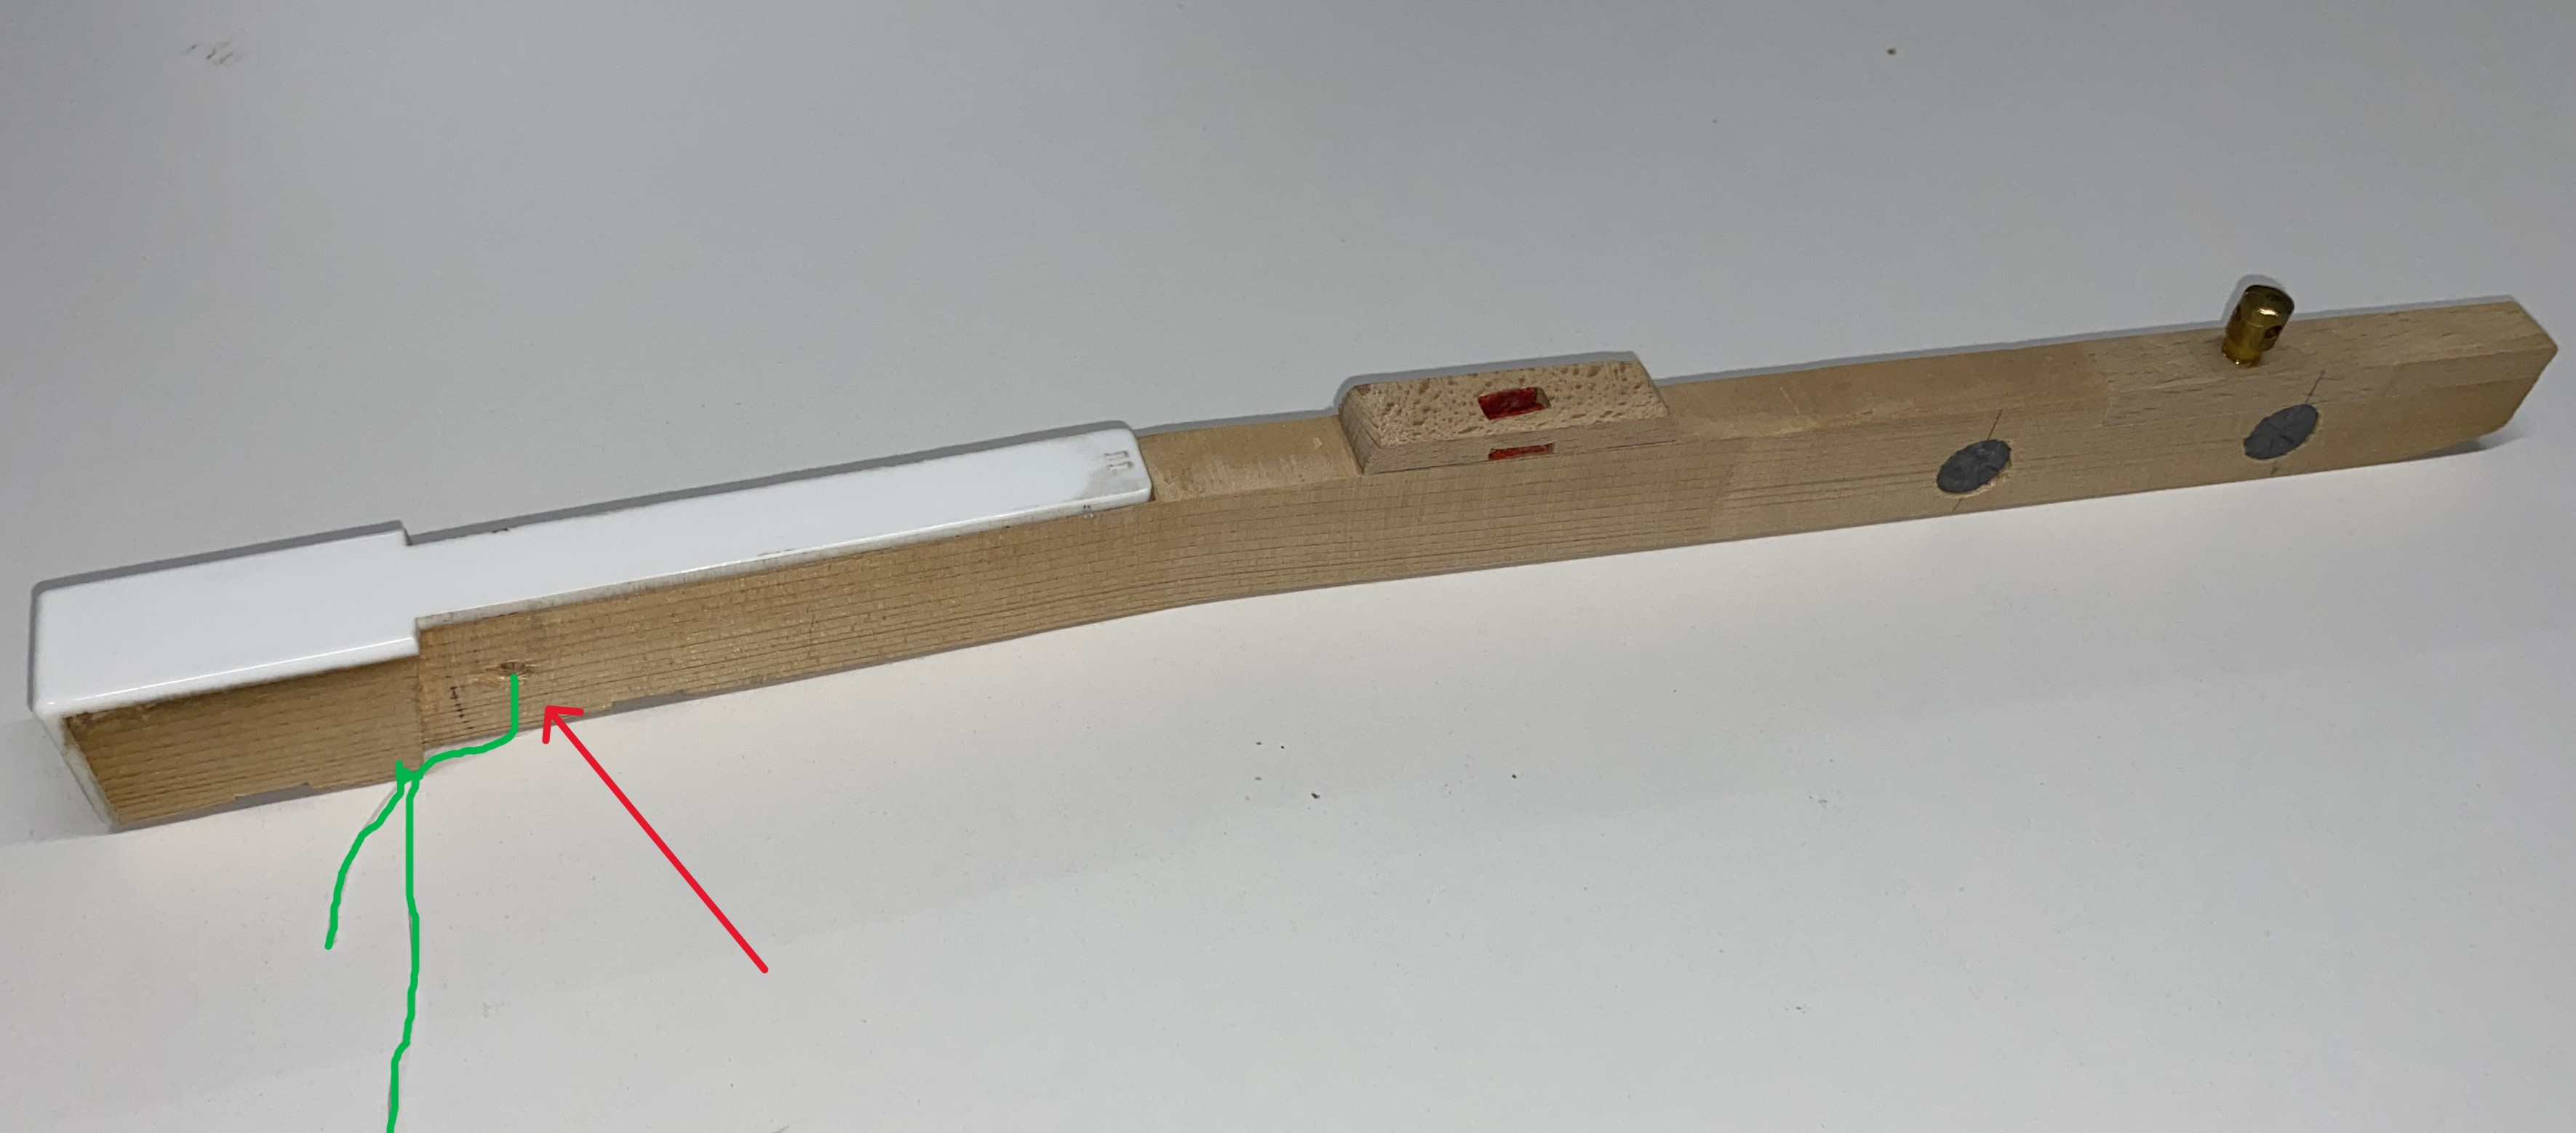
\includegraphics[width=8cm]{img/Taste_schraeg.jpg}
	\caption{Tastenbohrung}
\end{figure}


Anschließend wird jede Schnur jeweils durch ein senkrechtes Loch (rot in Abbildung \ref{fig:klaviatur} gekennzeichnet) im Klaviaturbalken (bzw. Tastenbrett),
worauf die Tasten liegen, in den Fußraum geführt.

\begin{figure}[htbp]
	\centering
	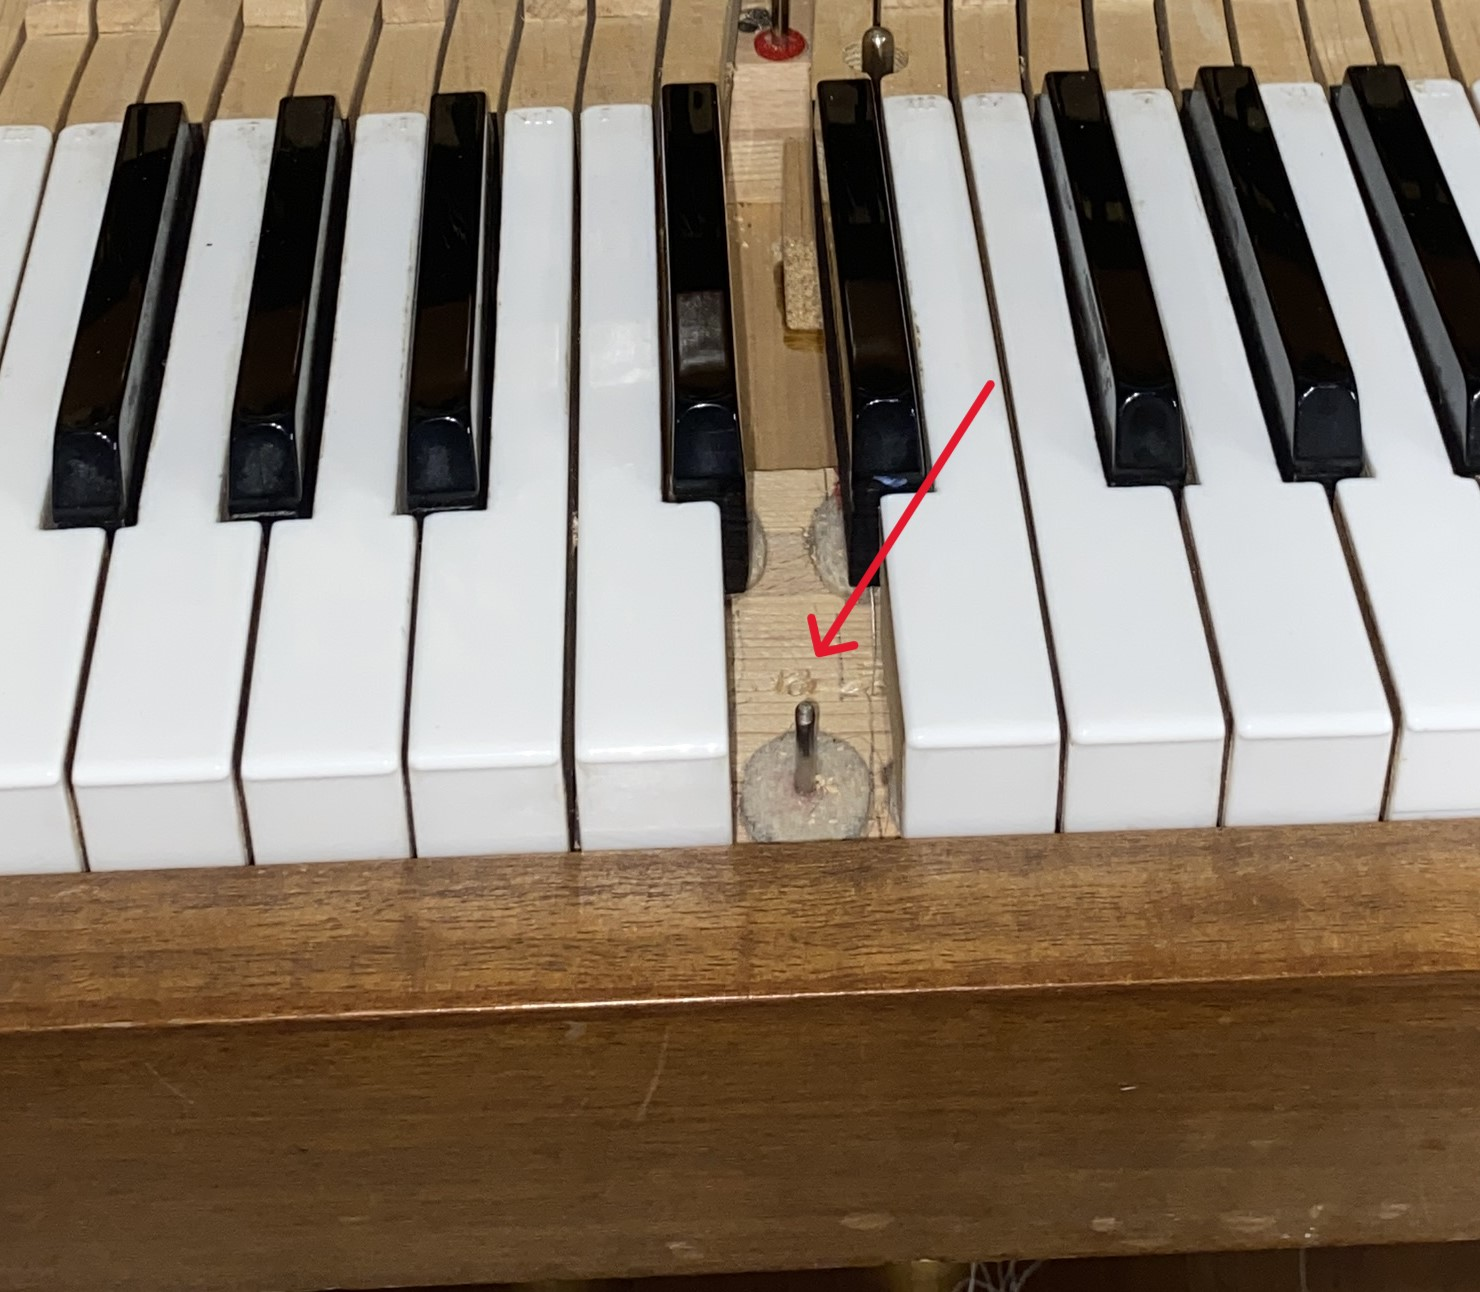
\includegraphics[width=5cm]{img/Klaviatur.jpg}
	\caption{Bohrung durch das Tastenbrett}
	\label{fig:klaviatur}
\end{figure}

Damit die Pianist:innen nicht durch Platzmangel im Beinbereich eingeschränkt sind,
werden die Seile entlang der Verkleidung zur unteren Frontplatte des Klaviers geführt. (siehe Abbildung \ref{fig:fussraum})


\begin{figure}[htbp]
	\centering
	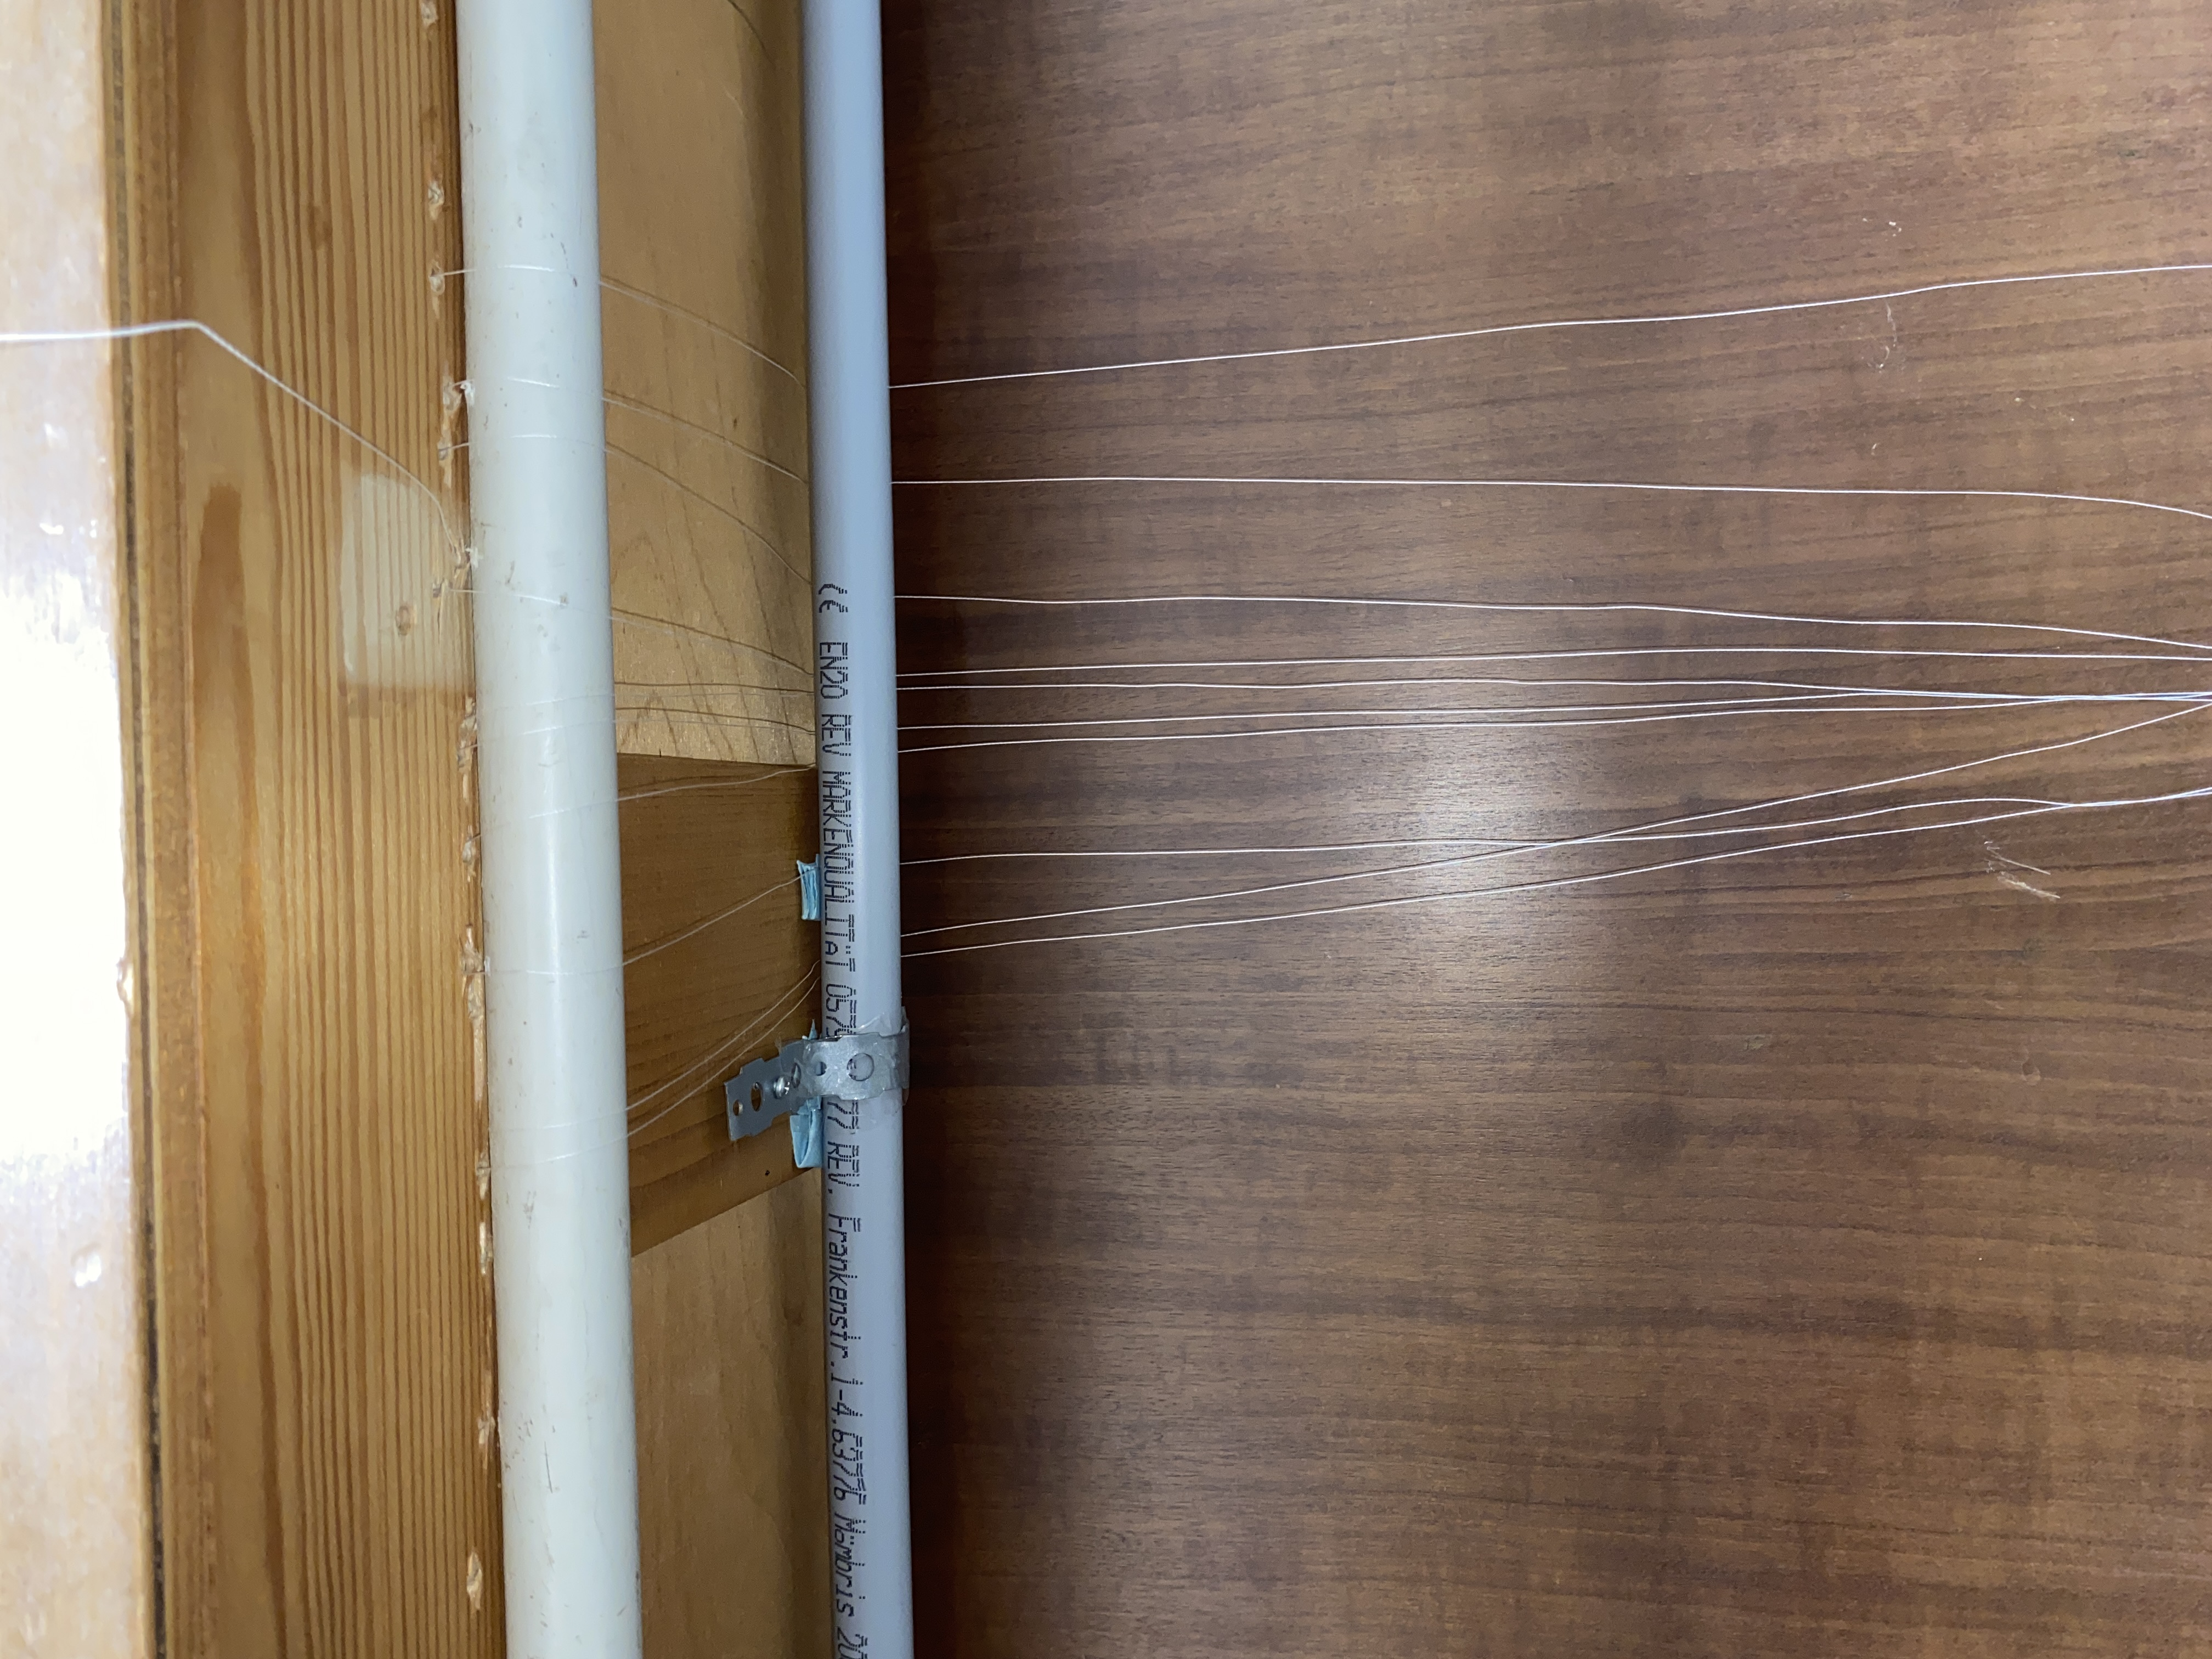
\includegraphics[width=5cm,angle=-90]{img/Fussraum.jpg}
	\caption{Fußraum des Klaviers}
	\label{fig:fussraum}
\end{figure}



Dort werden die Hubmagnete in zwei Reihen über die gesamte Breite befestigt. (siehe Abb. \ref{fig:BefestigungHubmagnete})

\begin{figure}[htbp]
	\centering
	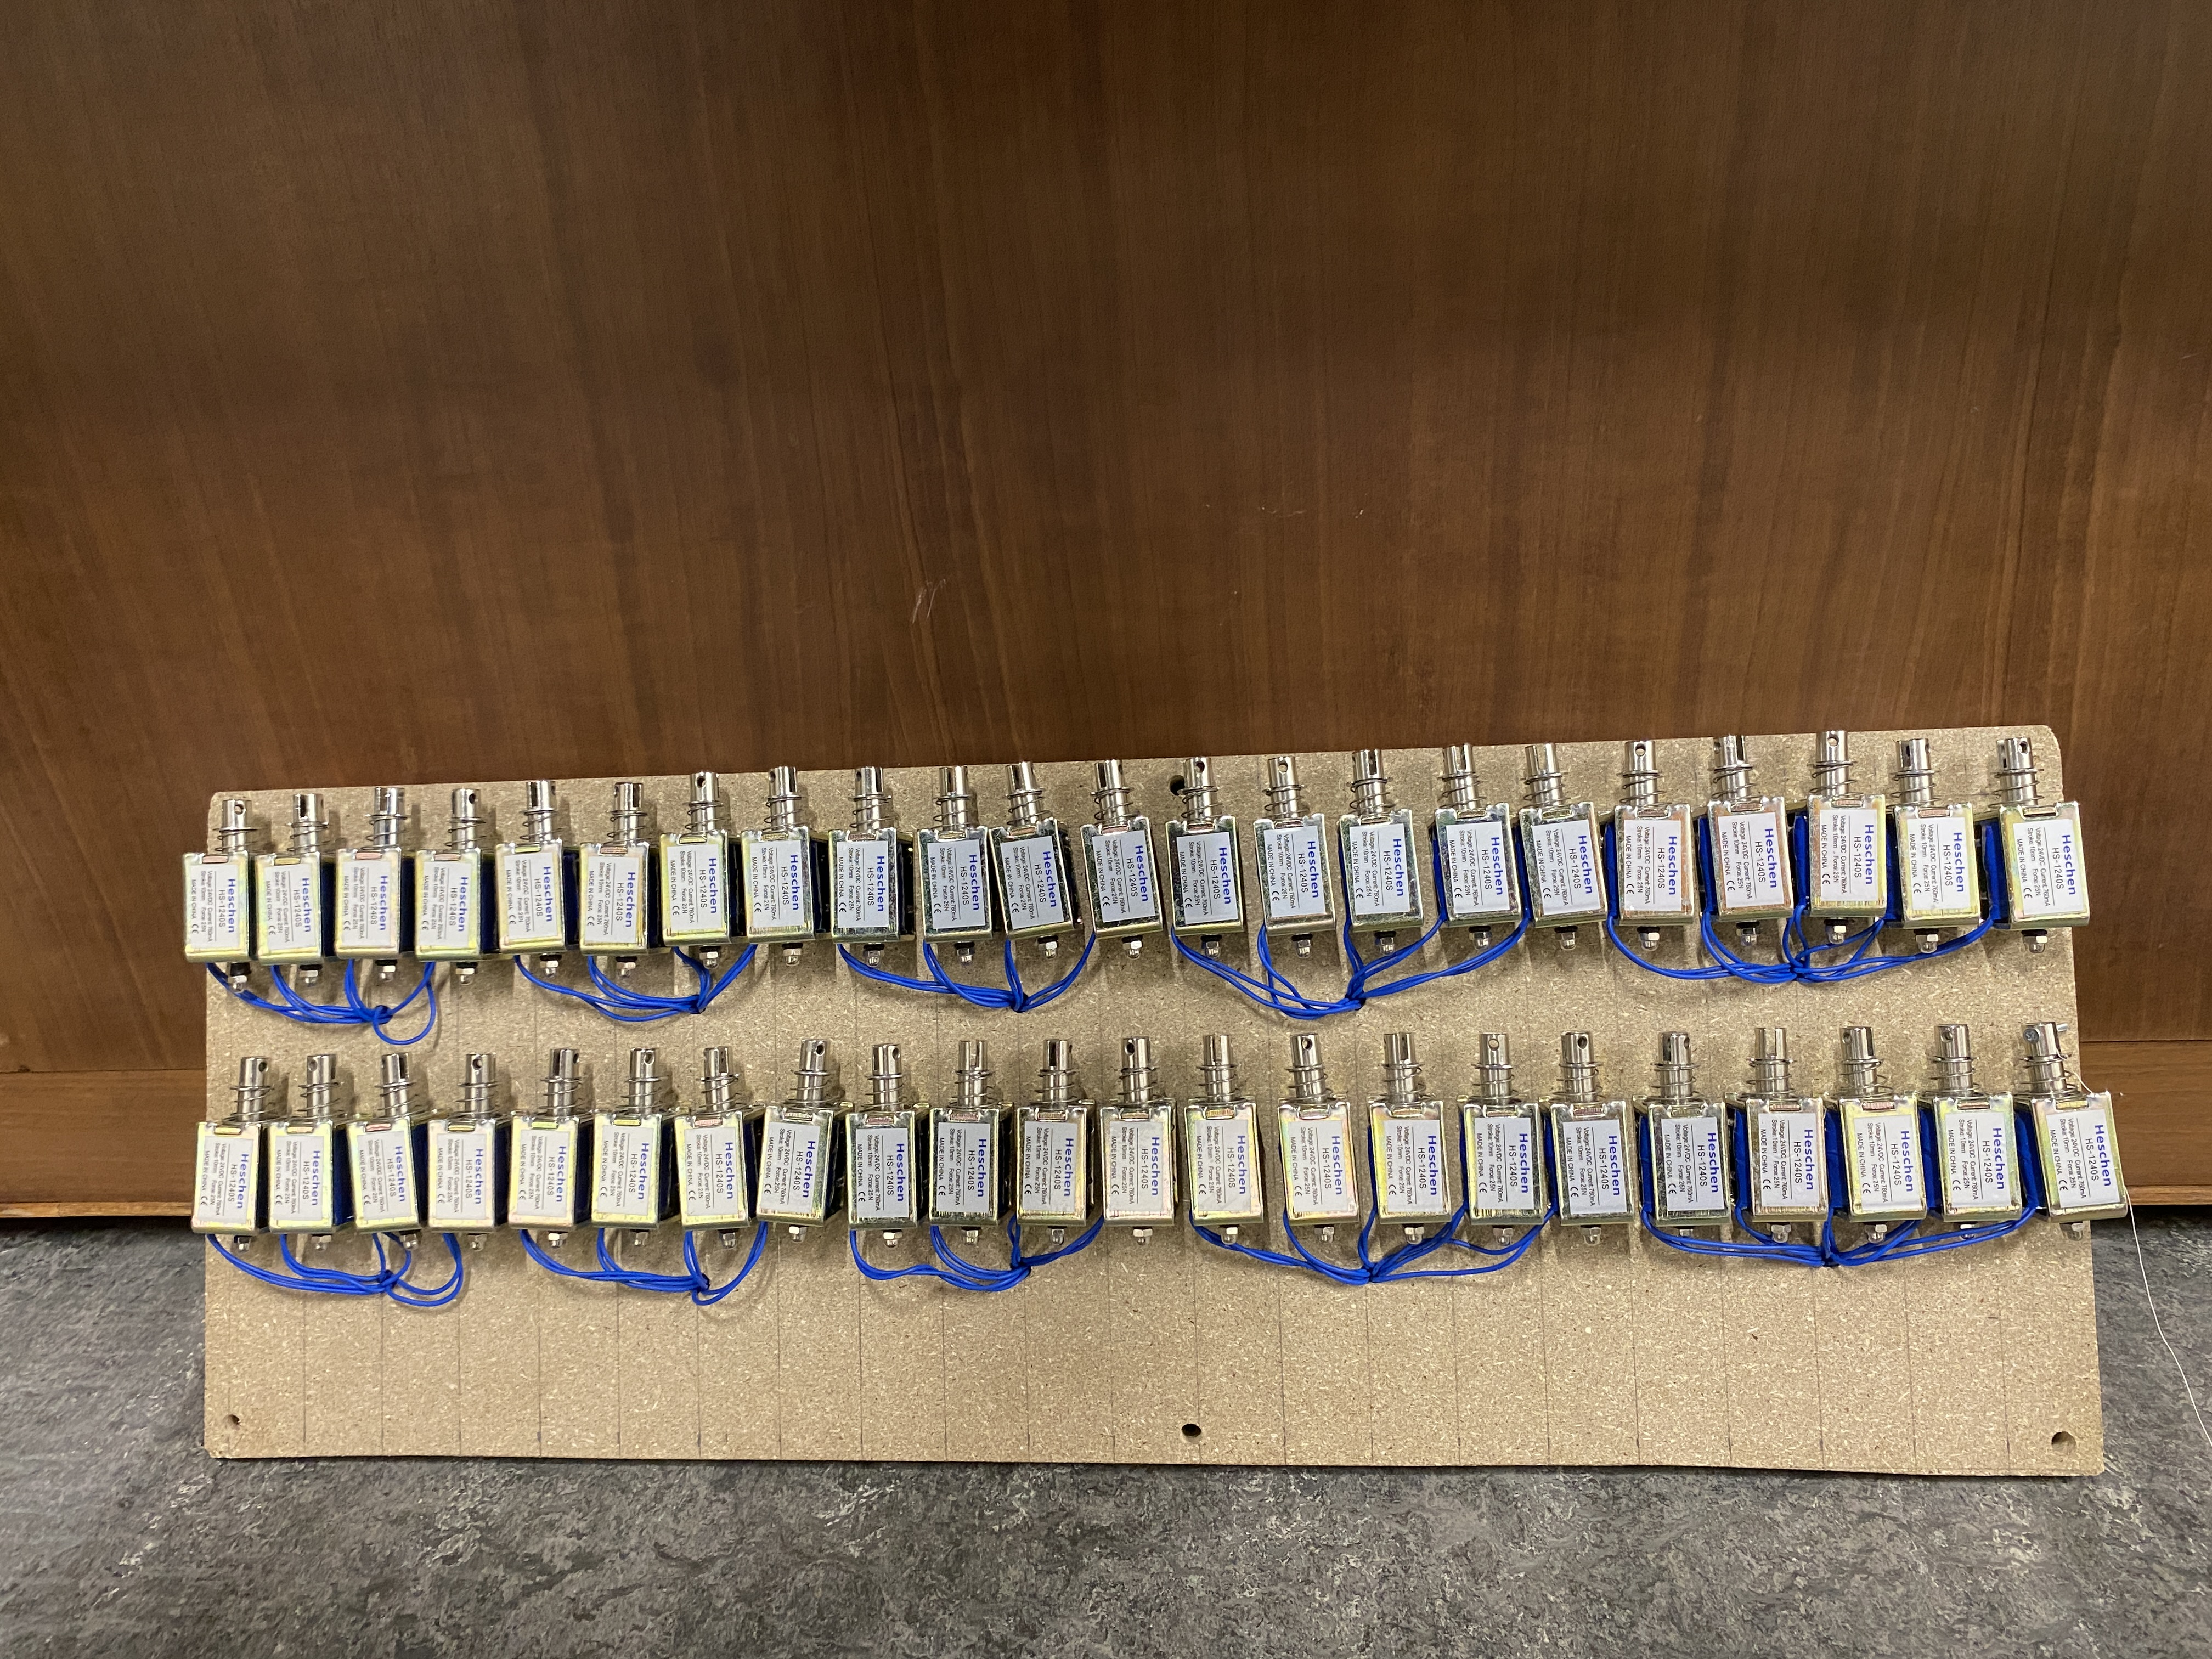
\includegraphics[width=5cm]{img/Magnetbrett.jpg}
	\caption{Befestigung der Hubmagnete}
	\label{fig:BefestigungHubmagnete}
\end{figure}
Um die Intensität des Tastendrucks zu steuern und die Haltbarkeit des Materials zu verlängern,
sollte die Reibung am Seil möglichst gering gehalten werden.
Dazu werden mittels Rohren, welche waagerecht unter dem Klaviaturbalken entlang der Löcher montiert werden, die Seile umgelenkt.

\textit{Anordnung der Aktuatoren}

Die Idee ist, die Hubmagnete entlang der Klaviatur zu befestigen, um die Tasten möglichst senkrecht nach unten ziehen zu können.
Hierfür müssen folgende Aspekte berücksichtigt werden:

\begin{enumerate}
	\item Breite der Hubmagnete
	\item Hitzeentwicklung
	\item Seilführung
	\item Stabilität
	\item Modularität
\end{enumerate}

Ein Hubmagnet hat die Maße 2,5 cm x 6 cm.
Das Tastenbrett für 88 Tasten ist allerdings nur 140 cm breit, wodurch pro Tastenansteuerung nur ca. 1,6 cm zur Verfügung stehen.
Bildet man zwei Hubmagnetreihen übereinander, hat jede Tastenansteuerung 3,20 cm Platz.

Durch die 7mm Abstand ist eine Wärmeabfuhr über die Luft in geringem Ausmaß möglich.
Ob dies ausreicht, muss in späteren Tests (siehe Kapitel \ref{tests}) ermittelt werden.

Alle Seile werden pro Hubmagnetreihe, parallel zwischen Tasten und Hubmagnete verbunden.

Die Hubmagnete direkt unter dem Tastenbrett zu befestigen wäre eine triviale Lösung würde allerdings auf Kosten der Stabilität und Funkionalität gehen.
Deshalb werden die Hubmagnete am Korpus des Klaviers (untere Frontplatte) befestigt.

Um die Austauschbarkeit der Komponenten zu verbessern, werden die Hubmagnete nicht direkt an der unteren Frontplatte,
sondern auf zwei Pressspanplatten (ca. 70 cm x 25 cm) befestigt, welche an vier Punkten mit dem Klavier verschraubt werden.


\textit{Optimierung der Seilführung}

Würde man die Seile direkt zu den Hubmagneten führen,
hätte man deutliche Hub-Verluste und könnte unter Umständen die Tasten nicht mehr ausreichend betätigen.
\newline
In den folgenden Abbildungen sind die seitliche Ansicht des Klaviers gezeichnet.
Dabei repräsentieren der schwarze/weiße Block jeweils eine schwarze/ weiße Taste.
Der grüne und pinke Strich stehen für das Seil, das mit dem Hubmagnet und dem Loch in der Taste verbunden ist.
Unten links sind die zwei übereinanderliegenden Solenoid-Reihen (blau) abgebildet.
Der schwarze Strich repräsentiert den Stab im Hubmagneten.
\newline
Abb. 3.1 zeigt den intuitiven Aufbau mit entspanntem Seil und ausgeschaltetem Solenoid.
Abb. 3.2 zeigt den selben Aufbau wie Abb. 3.1, nur, dass der Solenoid angezogen ist.

\begin{figure}[htbp]
	\centering
	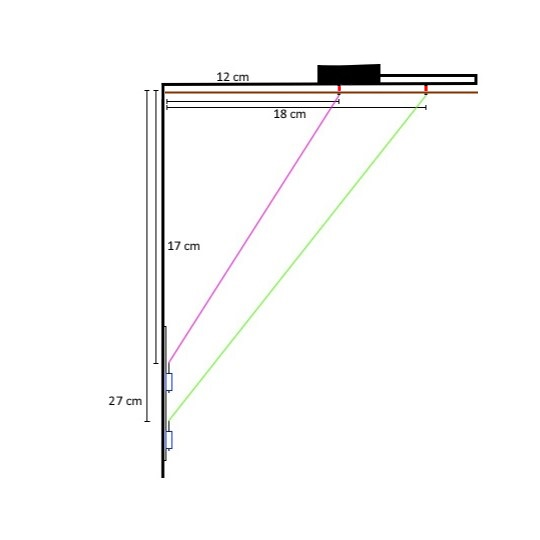
\includegraphics[width=8cm, height=10cm]{img/Umlenkung_locker}
	\caption{Taste locker ohne Umlenkung}
\end{figure}

\begin{figure}[htbp]
	\centering
	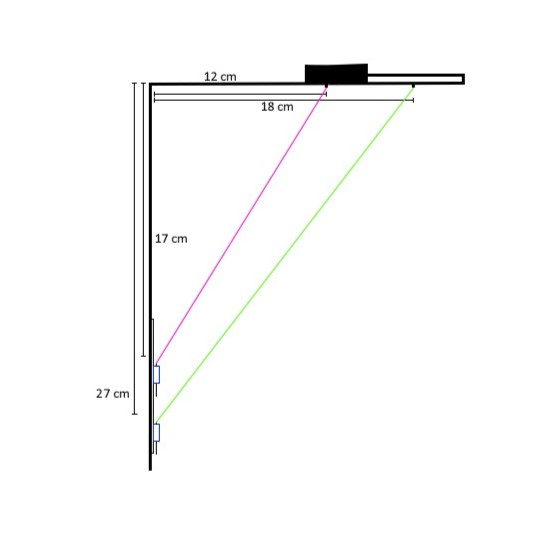
\includegraphics[width=8cm, height=10cm]{img/Umlenkung_gezogen}
	\caption{Taste gezogen ohne Umlenkung}
\end{figure}

\newpage

Mit diesem intuitiven Aufbau funktioniert das Betätigen der Taste nicht, da diese nicht weit genug heruntergezogen wird.
Um den gesamten Hub des Magneten zu Nutzen und an die Taste weiterzugeben wurden Umlenkungen eingebaut.
Mittels dieser Umlenkung (PVC-Rohr) werden die Seile so geführt, das sie senkrecht auf die Hubmagnete fallen.
Somit wurde die Tiefe, mit der die Taste gedrückt werden kann, wieder auf annähernd 1 cm (Hub des Magnets) erhöht werden.

\begin{figure}[htbp]
	\centering
	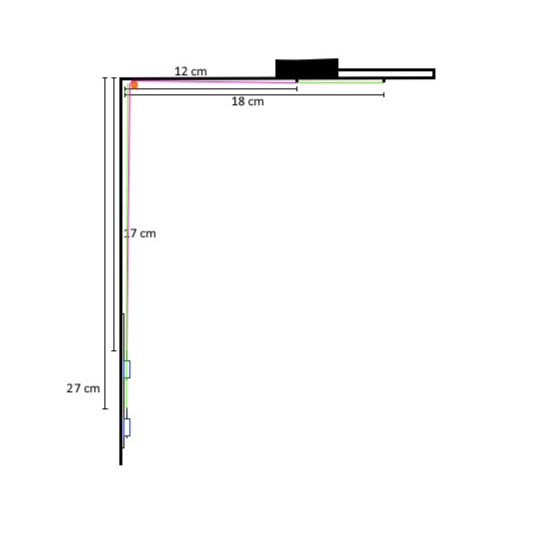
\includegraphics[width=8cm, height=10cm]{img/mitUmlenkung_locker}
	\caption{Taste mit Umlenkung}
\end{figure}


Dies kann man auch mathematisch beweisen:
\newline geg.:
\newline Strecke bis zur ersten Reihe Hubmagnete h1 = 17 cm
\newline Strecke bis zur zweiten Reihe Hubmagnete h2 = 27 cm
\newline Strecke bis zu den schwarzen Tasten t1 = 12 cm
\newline Strecke bis zu den weißen Tasten t2 = 18 cm
\newline Seil zur schwarzen Taste im entspannten Zustand $ht1_{entspannt}$
\newline Seil zu den weißen Tasten im entspannten Zustand $ht2_{entspannt}$
\newline $ht1_{entspannt}$ = $\sqrt {h1^{2} + t1^{2}}$ = 20.81 cm
\newline $ht2_{entspannt}$ = $\sqrt {h2^{2} + t2^{2}}$ = 32.45 cm
\newline $ht1_{gespannt}$ = $\sqrt {(h1 + 1) ^{2} + t1^{2}}$ = 21.63 cm
\newline $ht2_{gespannt}$ = $\sqrt {(h2 + 1)^{2} + t2^{2}}$ = 33.29 cm

Die Differenz zwischen $ht1_{gespannt}$ und $ht1_{entspannt}$ (bzw. ht2) beschreibt die Tiefe, die eine Taste gedrückt werden kann.
\newline Diese beträgt 0.82 cm, bzw. 0.84 cm.

\textit{Auswahl des Seils}

Wie eben erwähnt wird das Ziehen durch ein Seil ermöglicht.
Dafür wird ein leichtes, formbares, unelastisches und dehnungsresistentes Material benötigt, welches die Hubmagnete mit den Tasten verbindet.
Je leichter das Material ist, desto weniger wird die Genauigkeit der Kraftübertragung zwischen den Magneten und den Tasten verändert.
Durch die Formbarkeit kann der Knoten sehr eng an der Taste geschnürt werden, wodurch das Ansprechverhalten schneller erfolgen kann.
Da die Anschläge ruckartige Bewegungen sind, ist es wichtig ein unelastisches Seil zu verwenden.
Um häufiges Nachspannen oder Austauschen des Seils entgegenzuwirken, sollte dies so dehnungsresistent wie möglich sein.

\subsubsection{Nähgarn}

Als Erstes wurde Nähgarn, welches zur Hand war getestet.
Auch doppelt verlegt hielt es der ruckartigen Ziehbewegung (mit 25N) des Hubmagnetens nicht stand.
Vier Fäden funktionierten zu Beginn gut, leierten allerdings schnell aus.

\subsubsection{Nylonsaiten}

Als Nächstes wurde die g-Saite einer Gitarre verwendet.
Durch den höheren Durchmesser und das stärkere Material riss und leierte die Saite nicht aus.
Da die Saite kaum Flexibilität liefert, war die Befestigung an der Taste äußerst schwierig.
Beim Ziehen des Magnetes wurde erst die lockere Schlaufe an der Taste gestreckt, wodurch nicht der vollständige Hub des Magnetes auf die Taste übertragen werden.

\subsubsection{Angelschnur}

Aus Erfahrungen aus dem Angelbereich konnte schnell eine geeignetere Schnur gefunden werden.
Genauer handelt es sich um eine geflochtene Schnur aus Polyethylene.
Mit einem Durchmesser von 1.6 mm ist sie nicht nur sehr dünn und flexibel, sondern kann auch bis zu 7 kg standhalten.
Auch nach ausgiebigem Testen erfüllt die Angelschnur die Anforderungen.
Damit ist nun auch das Spielen des Forellenquintetts von Schubert ein leichtes.

\subsection{Klangdämpfung der Aktuatoren}
Die Hubmagnete machen beim Anschlagen laute \glqq klack\grqq {} Geräusche, welche von der Melodie des Klaviers ablenken.
Genauer handelt es sich um das den Metall-Anker, der gegen das Ende des Metall-Gehäuses stößt.
Auch hierfür gab es mehrere Ideen und Tests, um das Geräusch zu dämpfen:

\subsubsection{Isolierfolie}

Die erste Überlegung war die Auskleidung des Innenraums der Hubmagnete mit Isolierfolie.
Diese Idee wurde wieder verworfen, da das Wissen über die Hitzeentwicklung zu diesem Zeitpunkt noch zu gering war, um sicherzustellen, dass die Isolierung dem standhält.

\subsubsection{Gummi-Stopper}

Die nächste Idee war das Limitieren des Schlags durch Gummiringe (Dichtungsringe) zwischen Anker und dem äußeren Gehäuse.
Da für die Befestigung keine zufriedenstellende Lösung gefunden wurde, wurde auch diese Idee verworfen.
zurück schellen zu hoch, als dass wir die Klangdämpfung umsetzen würden.

\subsubsection{Schaumstoff}

Wie im Bild unten zu sehen, wurde die \enquote{Gummi-Stopper}-Idee durch den Einsatz von Schaumstoff leicht verändert.
+ Das Klopfgeräusch konnte vollständig verhindert werden.
- Durch den Schaumstoff kann 1 mm Hub nicht verwendet werden, weshalb nur noch 9 mm übrig bleiben.
- Der Aufbau optisch nicht ansprechend.

\begin{figure}[htbp]
	\centering
	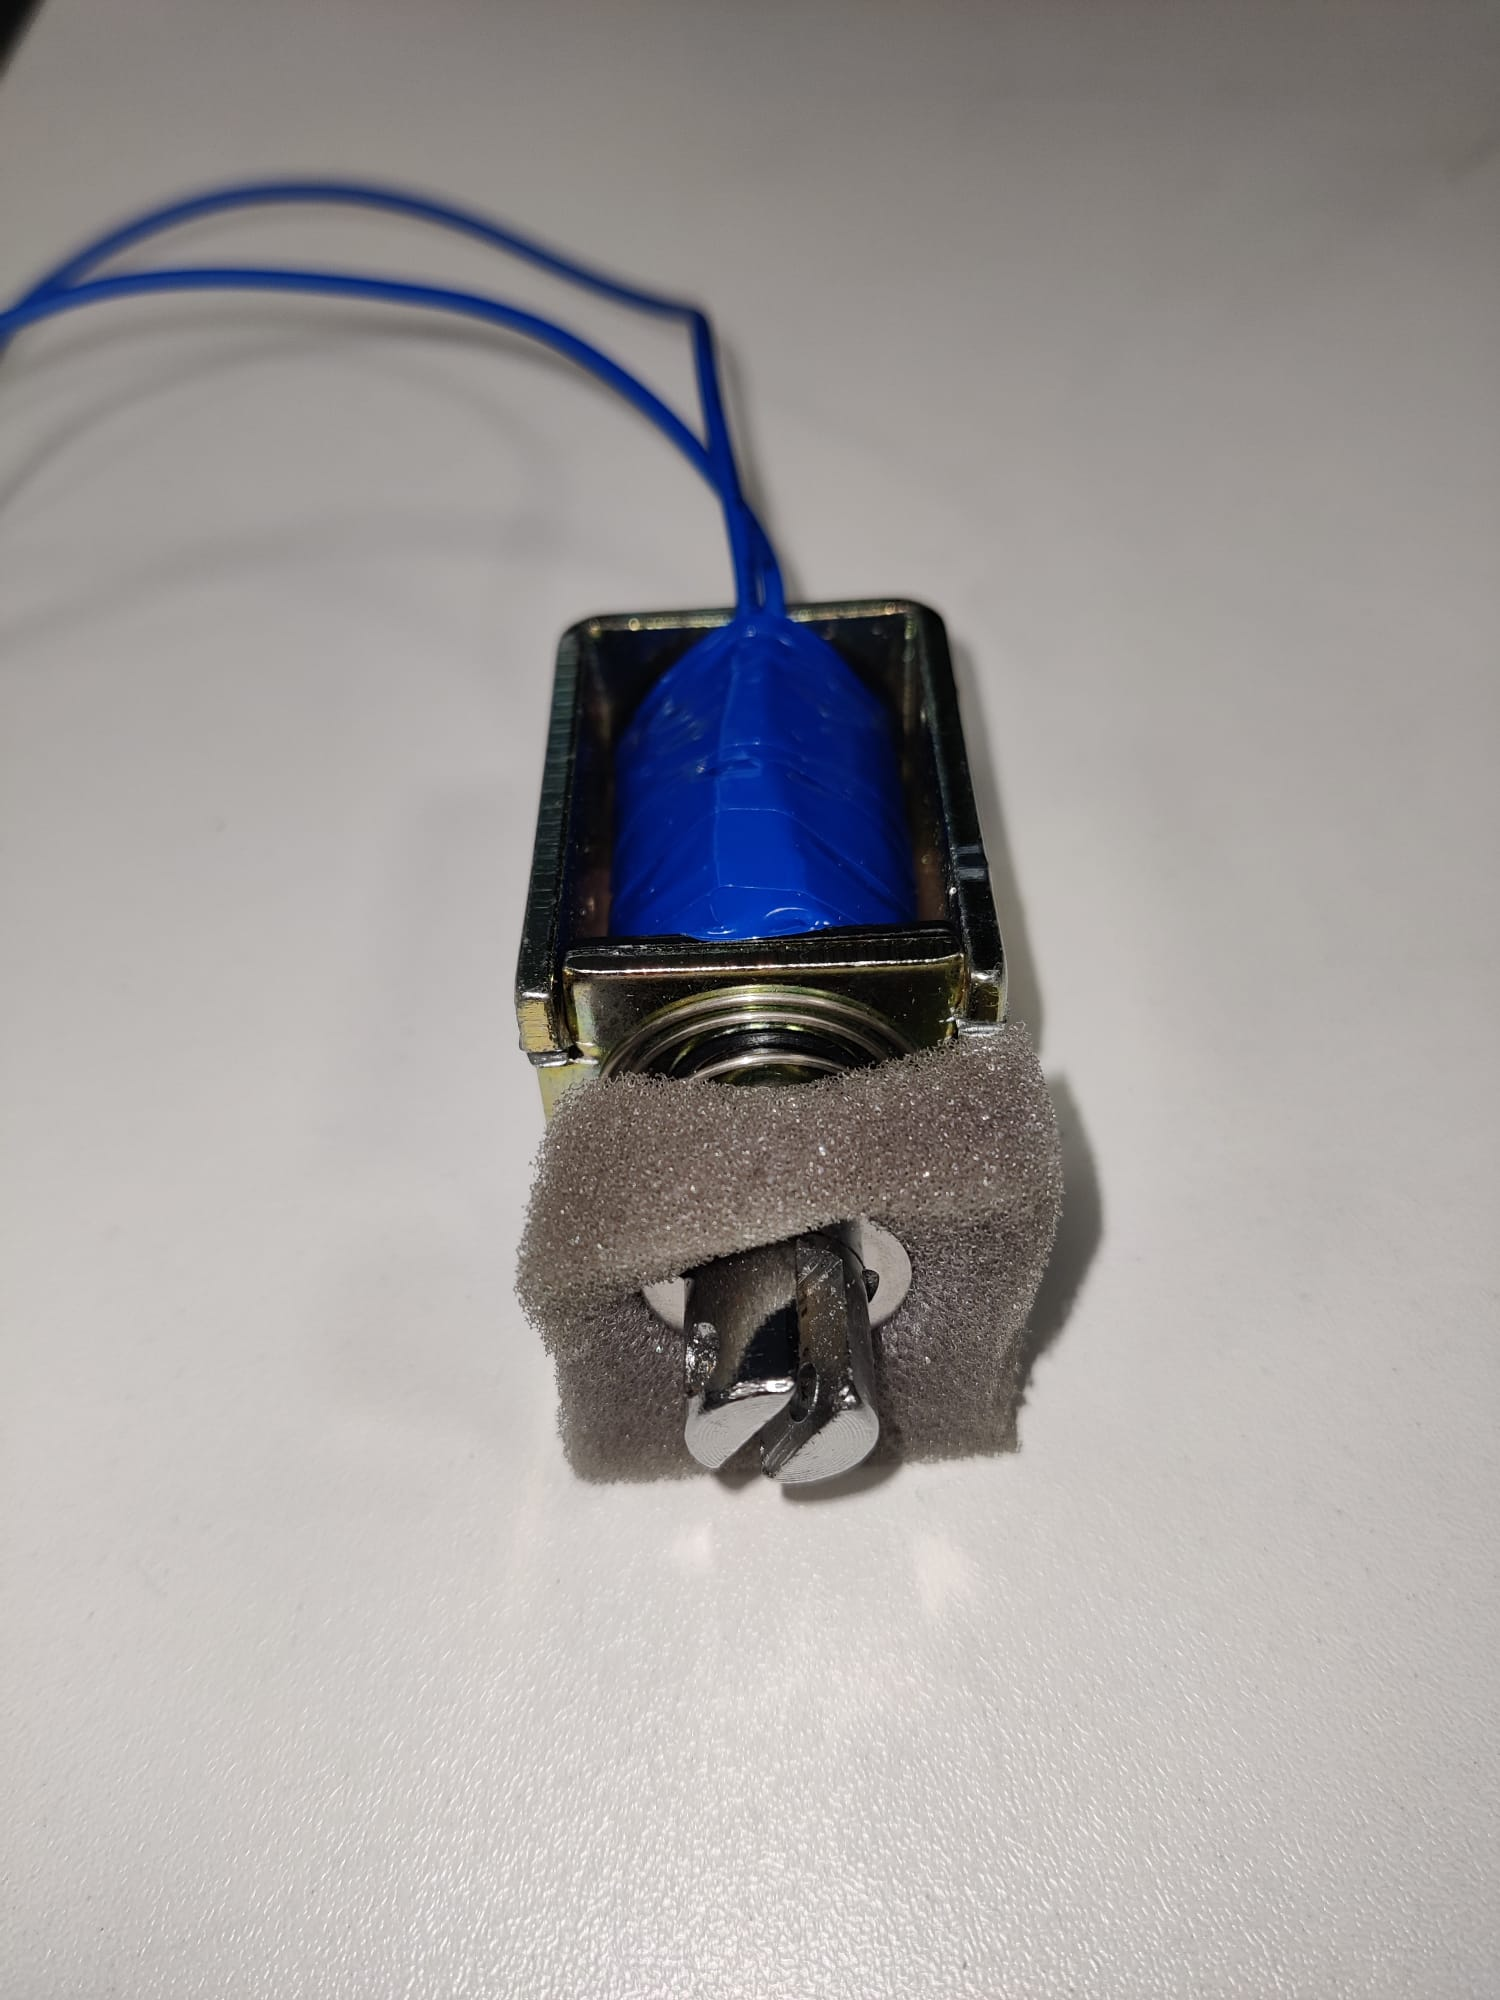
\includegraphics [width=4cm] {img/Daempfung_Schaumstoff}
	\caption{Hubmagnet: Dämpfung mit Schaumstoff}
\end{figure}

\subsubsection{Seil (2mm Durchmesser) um den Anker}

Um das "Problem" der schlechten Ästetik beim Schaumstoff zu beseitigen, wird nun ein 2mm dickes Seil im Inneren des Gehäuses um den Anker gewickelt. \newline
+ Auch hier konnte das Klopfen vollständig beseitigt werden \newline
+ Von außen sieht man keine Veränderung \newline
+ Bezogen auf die Hitzeentwicklung scheint das Seil nach den bisherigen Tests gut Stand zu halten. \newline
- Durch die Dicke des Seils, werden 2mm Hub nicht verwenden, weshalb nur noch 8mm übrig bleiben.

\begin{figure}[htbp]
	\centering
	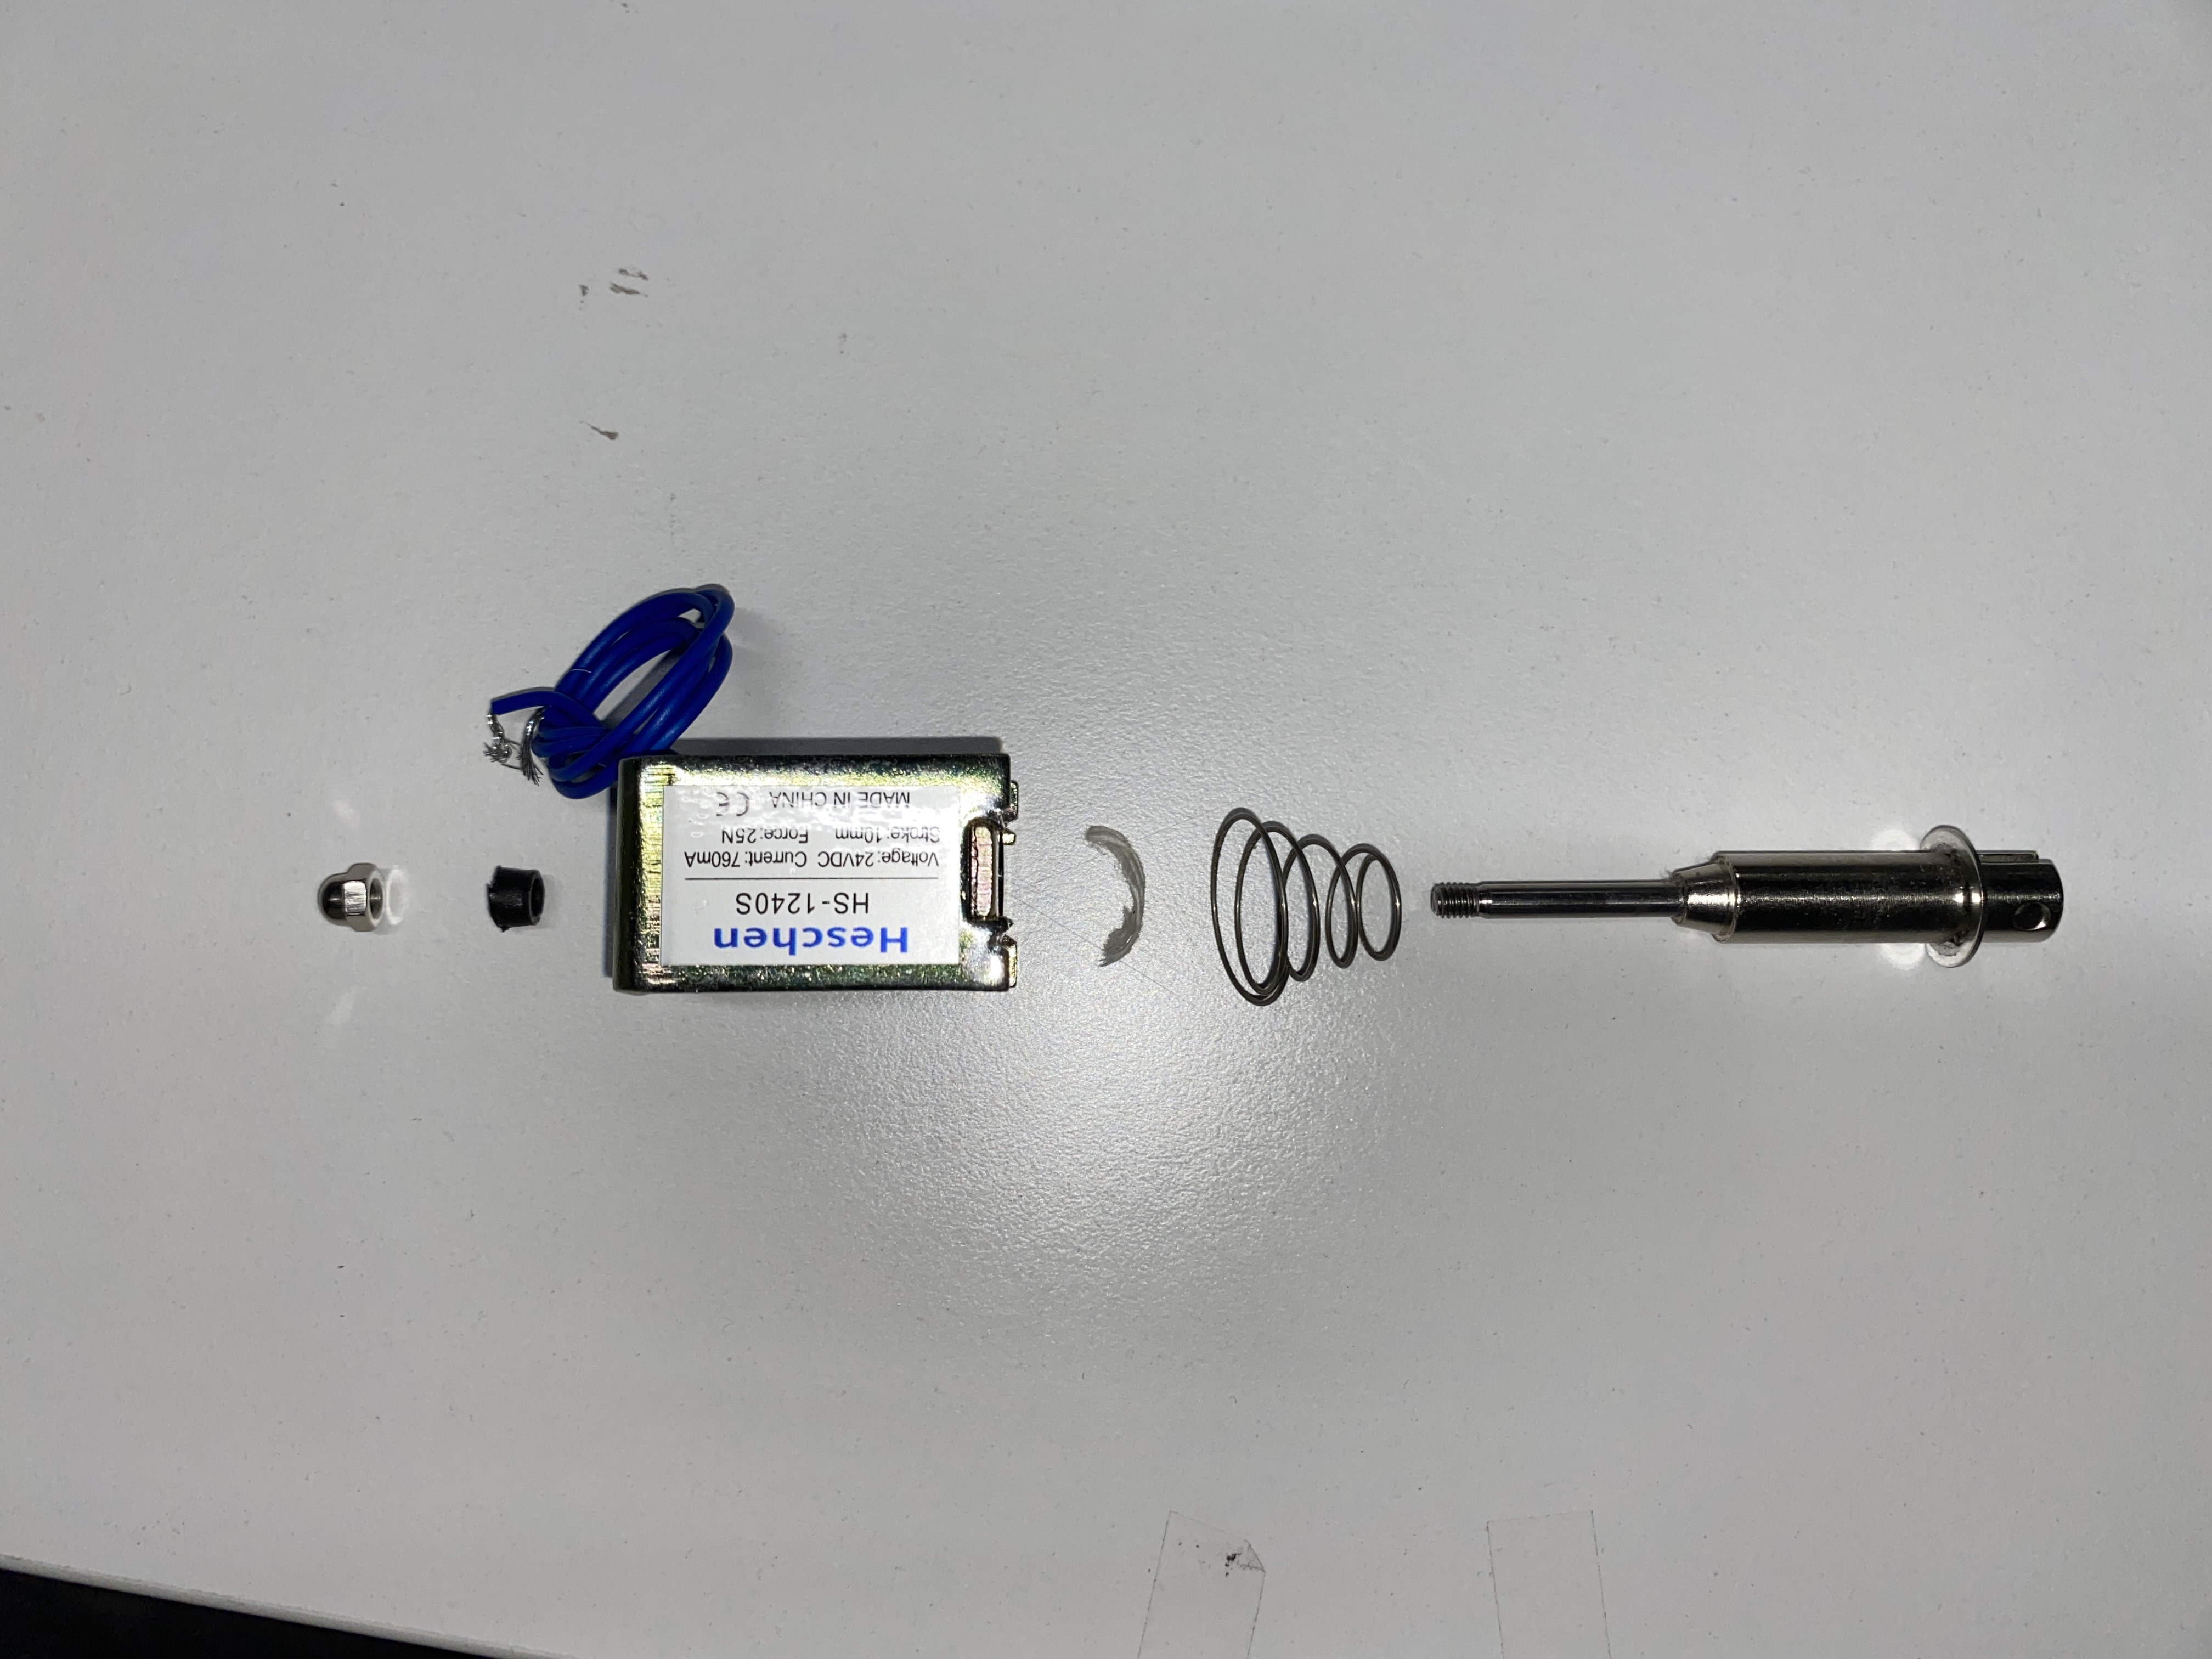
\includegraphics [width=4cm] {img/Hubmagnet_Seil_Daempfung.jpg}
	\caption{Hubmagnet: Dämpfung mit Seil}
\end{figure}

\section{Elektronik}\label{Vorgehen - Hardware}


\subsection{Mikrocontroller}\label{Ansteuerung}
Um die Signale des Programmes an die Aktuatoren weitergeben zu können, ist ein Mikrocontroller gut geeignet.
Auf dem Markt steht eine hohe Anzahl an Mikrocontrollern zur Verfügung, wobei für diese Arbeit ein Arduino und ein Rasperry Pi\footnote{Genau genommen handled es sich bei einem Rasperry Pi um einen Einplatinencontroller.} betrachtet wurden.

%Arduino Intro
\begin{minipage}{0.7\textwidth}
	\paragraph{Arduino}
	Bei einem Arduino handelt es sich um eine Plattform für die Entwicklung von elektronischen Prototypen.
	Er besteht aus einem Mikrocontroller-Board, das mit verschiedenen Sensoren, Aktuatoren und anderen elektronischen Komponenten verbunden werden kann.
	Der Arduino verfügt über digitale und analoge Ein- und Ausgangspins, die für die Interaktion mit Geräten verwendet werden können.
\end{minipage}
\begin{minipage}{0.3\textwidth}
	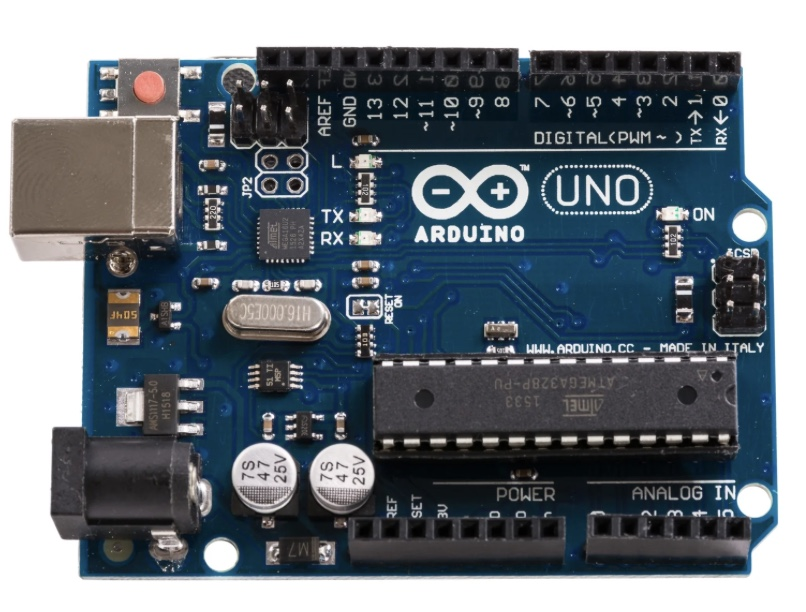
\includegraphics [width=\textwidth] {img/ArduinoR3}
\end{minipage}
\newline

%Pi Intro
\begin{minipage}{0.3\textwidth}
	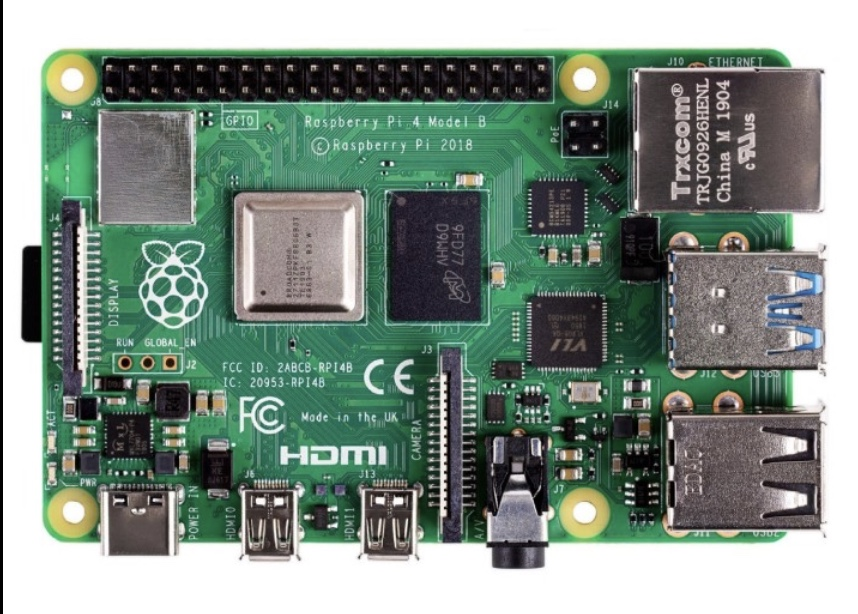
\includegraphics [width=\textwidth] {img/RasperryPi}
\end{minipage}
\begin{minipage}{0.7\textwidth}
	\paragraph{Rasperry Pi}
	Ein Rasperry Pi ist ein Einplatinencontroller, der auf einem ARM-Prozessor basiert.
	Er ist dafür konzipiert, eine breite Palette von Anwendungen zu unterstützen, von Prototypenbau bis IoT.
	% @Note(Val): "Im Gegensaz zum Arduino verfügt er über einen Prozessor" - falsch? der Arduino hat offensichtlich auch einen Prozessor...
	% @Cleanup(Val): Originaler Satz hier: (angepasst für Abgabe an Kruse für Email)
	% Im Gegensatz zum Arduino verfügt er über einen Prozessor und ist besonders für komplexe und rechenlastige Projekte geeignet.
	Im Gegensatz zum Arduino ist er besonders für komplexe und rechenlastige Projekte geeignet.
\end{minipage}
\newline

%Vergleich
% @Note(Val): Das war der originale Satz, aber der klang sehr komisch...: "Die Entscheidung für den verwendeten Mikrocontroller traf auf den Arduino."
Es wurde sich letztendlich für den Arduino entschieden.
Der Rasperry Pi stand vor allem aufgrund seiner höhere Speicherkapazität und Rechenleistung zur Diskussion, wodurch eine Komplexe Ansteuerungslogik möglich ist und ein Großteil des Programmes auf dem Rasperry Pi ausgeführt werden kann.
Allerdings ist er aufgrund seines Betriebssystems und einer erhöhten Latenz nicht für Echtzeit-Anwendungen bzw. Geschwindigkeitskritische Anwendungen ausgelegt.
Im Gegensatz dazu bietet der Arduino eine Echtzeitverarbeitung mit geringer Latenz.
Außerdem verfügt ein Arduino über eine recht simple Hardware-Interaktion - er ist darauf spezialisiert, die Hardware direkt anzusprechen und ist somit besser für Projekte geeignet, welche eine präzise Ansteuerung von Aktuatoren benötigt.
Zudem ist die Komplexität der Ansteuerung nicht so hoch, dass der Microcontroller über eine hohe Rechenleistung verfügen muss.

Für das Projekt wird spezifisch ein Arduino R3 verwendet. Bei der Auswahl des spezifischen Arduinos wurden der Arduino Uno, Nano und R3(auch: mega 2563) betrachtet.
Im Prinzip wäre jedes der Modelle für die Anwendung möglich, allerdings verfügt der R3 im Gegensatz zu den anderen beiden Modellen über mehr Speicherkapazitäten (256KB Flash Speicher
gegenüber der 32KB vom Arduino Uno und den 16KB des Arduino Nanos).
Der Arduino Uno verfügt zwar über mehr Ports, allerdings bringt dies keinen Mehrwert, da die Anzahl der benötigten Ausgänge auch bei einem Arduino Uno nicht erreicht werden
(siehe Kapitel \ref{output}).
Der Arduino R3 bietet - wie die anderen beiden Modelle auch - \ac{PWM} Pins, die im Rahmen des Projekts genutzt werden können.

\subsection{Pulsweitenmodulation (PWM)}\label{PWM}
Zur Vollständigkeit wird in diesem Abschnitt das Prinzip der Pulsweitenmodulation erläutert.
Oftmals ist bei der Ansteuerung der Aktuatoren nicht die gesamte Versorgungsspannung erwünscht bzw. gebraucht.
In diesen Fällen muss die anliegende Spannung varriiert werden, damit die Spannung am Ziel dem gewünschten Wert entspricht.
Angenommen es ist eine Spannung von 2.5V erwünscht, wobei die Vollversorgungsspannung 5V beträgt.
Das Signal kann dafür die Hälfte der Zeit ausgeschaltet werden, womit zwischen 0V und den vollen 5V durchschnittlich insgesamt 2.5V anliegen.
Je höher die Frequenz zwischen an- und ausschalten des Signals eingestellt wird, desto weniger wird diese ``künstlich'' simulierte Halbierung wahrgenommen.

\ac{PWM} bedient sich im Grunde genau dieser Technik.
Dabei wird die Zeitdauer eines digitalen Signals variiert wird, um einen durchschnittlichen Wert zu erzeugen.
Bei den \ac{PWM}-Ausgängen wird die Pulsweite - die Dauer der Einschaltzeit - des Signals angepasst, um die gewünschte Spannung zu erreichen.

\begin{figure}[htbp]
	\centering
	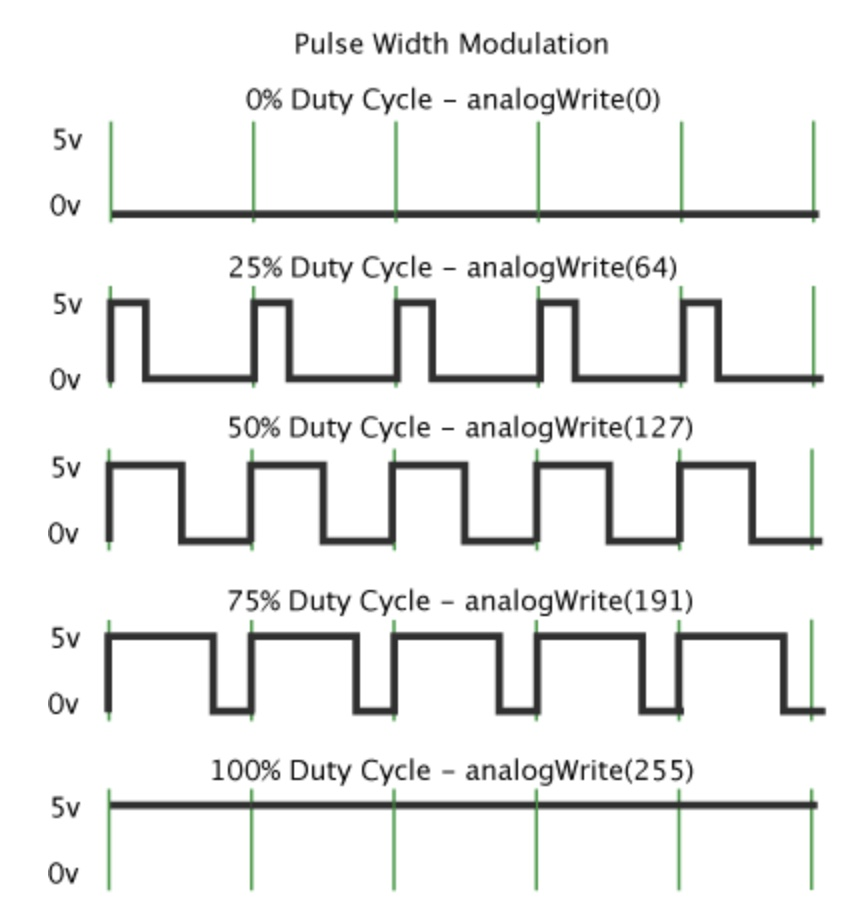
\includegraphics [width=13cm, height=8cm] {img/pulsweite}
	% @Note(Val): Quelle des Bilds fehlt hier noch
	\caption{Pulsweite}
	\label{fig:pulsweite}
\end{figure}

Spezifischer ausgedrück passiert folgendes:
Eine digitale Steuerung wird verwendet, um eine Rechteckwelle - ein Signal das zwischen Ein und Aus umgeschaltet wird - zu erzeugen.
Dieses Ein-Aus-Muster kann Spannungen zwischen der vollen Versorgungsspannung und 0V simulieren.
Dabei wird der Anteil der Zeit geändert, für den das Signal eingeschaltet ist im Vergleich zur Zeit, die das Signal ausgeschaltet ist.
Um unterschiedliche analoge Werte zu erhalten, wird die Pulsweite geändert bzw. moduliert.
Wenn dieses Ein-Aus-Muster zum Beispiel schnell genug mit einer LED wiederholt wird, resultiert daraus eine konstante Spannung zwischen 0 und Vcc, die die Helligkeit der LED steuert.
% @Note(Val): was ist "Vcc" hier?

% @Note(Val): Hier wechselst du von Ein, Aus zu HIGH, LOW. Einheitliche Benennung wäre hier sinnvoller
Auf den Arduino bezogen sieht die Umsetzung eines \ac{PWM} Signals wie folgt aus:
Ein Taktsignal gelangt in die entsprechende Clock.
Die Clock stellt den entsprechenden \ac{PWM}-Modus ein.
Dabei werden zwei wichtige Werte gesetzt:
Der erste bestimmt, wann das Signal von HIGH auf LOW umschaltet, während der zweite bestimmt, wann es zurückkommt.
Das Verhältnis zwischen HIGH und LOW wird als Tastverhältnis bezeichnet und bestimmt die Helligkeit unserer LED bzw. die Stärke, mit welcher der Hubmagnet anschlägt.
Je länger die Ausgabe im HIGH-Zustand bleibt, desto schneller erfolgt der Tastenanschlag.

Neben dem Tastverhältnis, also das Verhältnis der Einschaltzeit zur Periodendauer, welches oft in Prozent ausgedrückt wird, ist auch die Resolution (de: Auflösung) ein variierbarer Parameter.
Die Resolution bezieht sich auf die Anzahl der möglichen diskreten Werte, die das Signal annehmen kann.


\subsection{Vermehrung der Ausgänge}\label{output}
Da ein Klavier über 88 Tasten verfügt, müssen 88 Aktuatoren angesteuert werden. Ein Arduino hat keine 88 \ac{PWM}-Ports, daher
müssen die Signale über eine Erweiterung der Ausgänge an die Motoren weitergegeben werden. Dafür gibt es mehrere Möglichkeiten,
wobei in dieser Arbeit 2 im Detail betrachtet wurden:

\begin{enumerate}
	\item Schieberegister
	\item Aktuator-Matrix
\end{enumerate}

% Wäre es smart zu erwähnen was es noch für Möglichkeiten gibt? Also Arduino Mega muss ich soweiso erwähnen, aber z.B
% Shields verbinden oder mehrere Arduinos nutzen weil das haben wir ja kurz überlegt und dann relativ schnell verworfen

\paragraph{Schieberegister}
Ein Schieberegister ist ein integrierter Schaltkreis, der zur Speicherung und sequenziellen Verschiebung von
Datenbits verwendet wird.\newline
Das grundlegende Prinzip eines Schieberegisters ist, dass Datenbits seriell in das Register eingegeben und dann
sequenziell aus dem Register ausgegeben werden können.
Dies geschieht durch die Verwendung von Taktimpulsen, die das Verschieben der Bits steuern.\newline
Schieberegister bestehen aus einer Reihe von Flip-Flops.
Ein Flip-Flop kann als ein einfacher Speicher betrachtet werden, der binäre Informationen speichert und je nach
Eingangssignal den Zustand 1, 0, oder einen \enquote{Flip}-Zustand annimmt.
Diese FlipFlops sind so verbunden, dass sie Daten in einer bestimmten Reihenfolge speichern und weitergeben können.

Um 88 Ausgänge mit Hilfe von Schieberegistern, die von nur 3 \ac{PWM}-Pins des Arduinos agesteuert werden, umzusetzen,
können 11 8-Bit-Schieberegister  - also Schieberegister mit 8 Ausgängen - verwendet werden.
\paragraph{74HC959 Schieberegister}
In dieser Arbeit wird spezifisch ein 74HC959 Schieberegister betrachtet. Dieses hat folgenden Aufbau:
\begin{minipage}{0.4\textwidth}
	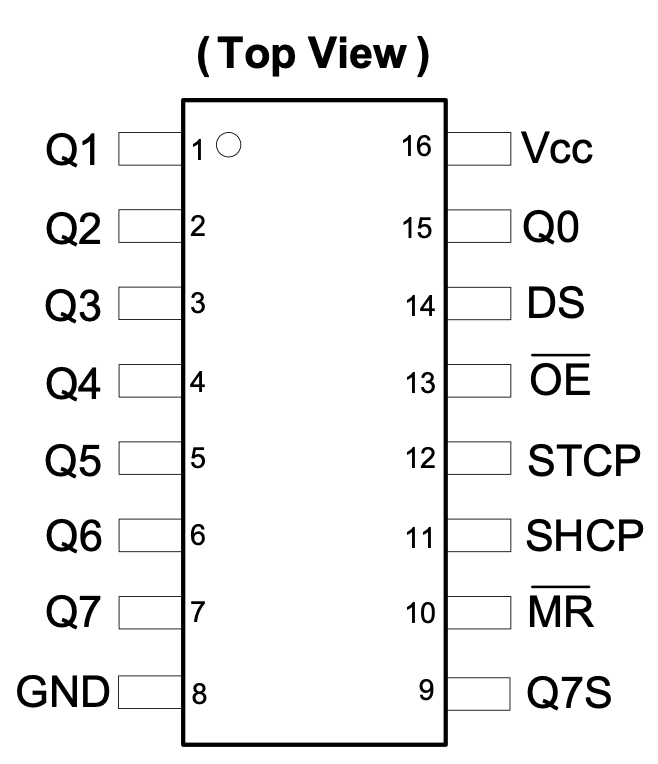
\includegraphics [width=0.4\textwidth] {img/Schieberegister}
\end{minipage}
\begin{minipage}{0.6\textwidth}
	\begin{enumerate}
		\item Q0-Q7: Ausgänge (parallelgeschaltet)
		\item Vcc: Anschluss Versorgungsspannung (+)
		\item Gnd: Anschluss Versorgugsspannung (-)
		\item DS: Data Signal, serieller Dateneingang
		\item OE: Output Enable, zur Aktivierung der Ausgänge
		\item SHCP: Shift Clock, Clock-Eingang zur Übernahme Data Signals in Schieberegister
		\item STCP: Store Clock, Wechsel Low auf High kopiert Inhalt des Schieberegister in Ausgaberegister
		\item MR: Master Reset, leerung Schift-register
		\item Q7S: Überlauf für Kaskadierung
	\end{enumerate}
\end{minipage}

Vorteile des Schieberegisters:\newline
Nachteile des Schieberegisters:
% @Note(Val): Wäre doch eigentlich eine "Aktuator-Matrix" oder "Magnet-Matrix", weil wir ja keine Motoren haben, oder?
\paragraph{Aktuator-Matrix}
% @TODO(Jay): Picture Matrix and use muster to explain it for magnets
Die Aktuator-Matrix ist einer LED-Matrix nachgeahmt.
In einer Matrix, werden zwei Reihen nach folgendem Muster an Ports angeschlossen:
$$
\begin{pmatrix}
	(11) & (12) & (13) & (14) & (15) & (16) & (17) & (18) \\
	(21) & (22) & (23) & (24) & (25) & (26) & (27) & (28) \\
	(31) & (32) & (33) & (34) & (35) & (36) & (37) & (38) \\
	(41) & (42) & (43) & (44) & (45) & (46) & (47) & (48) \\
	(51) & (52) & (53) & (54) & (55) & (56) & (57) & (58) \\
	(61) & (62) & (63) & (64) & (65) & (66) & (67) & (68) \\
	(71) & (72) & (73) & (74) & (75) & (76) & (77) & (78) \\
	(81) & (82) & (83) & (84) & (85) & (86) & (87) & (88)
\end{pmatrix}
$$

Eine LED-Matrix besteht aus einer Anordnung von LEDs in Zeilen und Spalten.
Jede LED kann unabhängig von den anderen ein- oder ausgeschaltet werden.\newline
Eine LED-Matrix sieht im Allgemeinen so aus:\newline
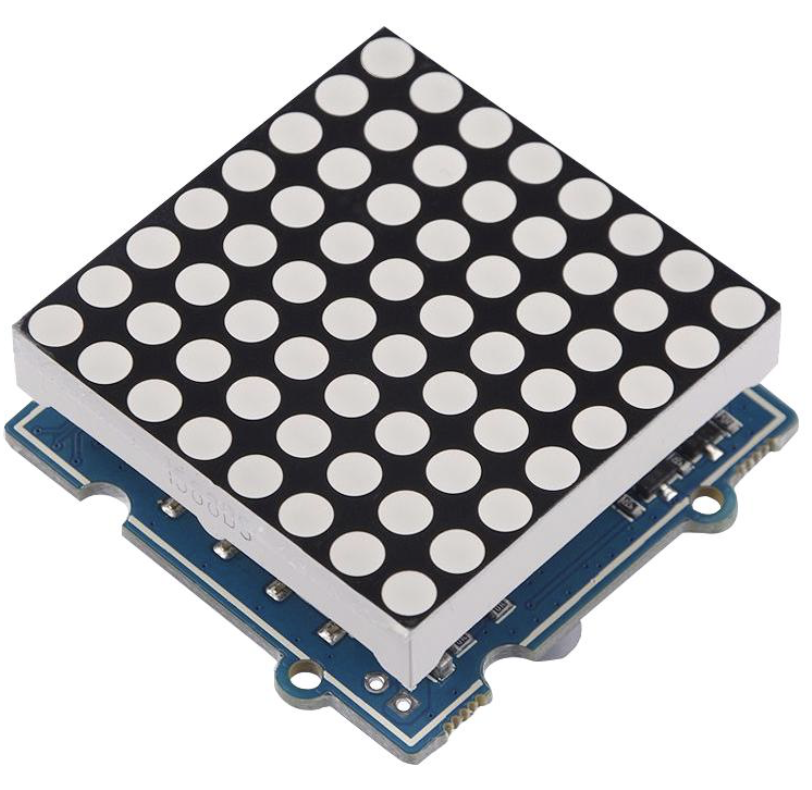
\includegraphics[width=0.45\textwidth]{img/LED-Matrix}
Die Steuerung der Matrix kann mit oder ohne Multiplexing erfolgen.
Prinzipiell wird jede Zeile der Matrix nacheinander aktiviert, während die
entsprechenden LEDs in den Spalten gleichzeitig eingeschaltet werden.
Durch schnelles Wechseln zwischen den Zeilen mithilfe von \ac{PWM} erscheint es den Betrachter:nnen, als ob alle LEDs
gleichzeitig leuchten würden, obwohl sie tatsächlich nacheinander aktiviert werden.\newline
%ohne Multiplexer
Matrix ohne Multiplexer:\newline
Bei einer LED-Matrix ohne Multiplexer werden die LEDs direkt über die GPIO-Pins (General Purpose Input/Output) des
Mikrocontrollers angesteuert. Jede LED ist einzeln mit einem Pin des Mikrocontrollers verbunden. Um die LEDs anzusteuern,
muss der Mikrocontroller jeden Pin einzeln aktivieren oder deaktivieren, um die entsprechende LED ein- oder auszuschalten.
Hierbei werden viele Pins benötigt, um die gesamte Matrix anzusteuern, was besonders bei größeren Matrizen unpraktisch
sein kann. Zum Beispiel erfordert eine 8x8-Matrix 64 Pins, was für viele Mikrocontroller zu viel sein kann. \newline
%Todo(Jay) add picture from Tinkercad
%mit Multiplexer
%Was ist ein Multiplexer, warum hilft er bei Martix wie sieht allg Schaltung aus?
Matrix mit Multiplexer: \newline
Ein Multiplexer (Beziehungsweise ein Demultiplexer) ist eine Schaltung, die es ermöglicht, mehrere Signale auf einem
einzelnen Kanal zu multiplexen (kombinieren) und dann selektiv zu demultiplexen (trennen)
Der Schaltkreis basiert auf einfachen Logik gattern.
In Bezug auf eine LED-Matrix bedeutet dies,
dass anstatt jeden einzelnen Pin der Matrix direkt mit einem GPIO-Pin des Mikrocontrollers zu verbinden, nur wenige Pins
benötigt werden, um die Matrix anzusteuern.
Der Vorteil des Multiplexers - die effizientere Ressourcennutzung - kommt allerdings mit einer komplexeren Schaltung und
möglichen Latenzen einher.
% TODO(Jay): Picture from Tinkercad

\paragraph{Entscheidungsfindung}
Nach weiterer Evaluation der Matrix schien es aus mehreren Gründen schwer möglich, das Prinzip von LEDs auf Aktuatoren
zu übertragen, weswegen die Entscheidung auf die Verwendung von Schieberegistern fiel. \newline
Eine LED-Matrix wird, wie bereits erklärt,
typischerweise durch PWM angesteuert, um den Eindruck zu erwecken, dass alle
LEDs gleichzeitig leuchten, obwohl sie tatsächlich nacheinander aktiviert werden. Dieses Prinzip funktioniert gut für LEDs,
da sie einen langsamen Reaktionsmechanismus haben und das menschliche Auge träge ist. Da die Aktuatoren via PWM
angesteuert werden,
Allerdings gibt es einige Gründe,
warum dieses Prinzip möglicherweise nicht sinnvoll ist, wenn man präzise Aktuatoren durch dasselbe Prinzip ansteuern
möchte:
\begin{enumerate}
	\item Stromversorgung und Energieeffizienz: LED-Matrizen werden oft mit einer relativ niedrigen Leistung betrieben, da
	LEDs im Vergleich zu Aktuatoren weniger Strom verbrauchen. Aktuatoren benötigen eine höhere Stromversorgung,
	um eine ausreichende Leistung für den Betrieb zu gewährleisten. Die Schaltung, die für eine LED-Matrix optimiert ist,
	könnte möglicherweise nicht die erforderliche Leistung für die Aktuatoren liefern.
	\item Interferenz und ungenaue Steuerung durch die Matrixstruktur: Bei der Verwendung einer Aktuatoren-Matrix über PWM
	könnte es zu Interferenzen kommen, die die Präzision der Steuerung beeinträchtigen. Da die PWM-Signale zeilenweise
	multiplexiert werden, kann es vorkommen, dass die PWM-Signale nicht mit der benötigten Stärke für jeden Aktuator geliefert
	werden. Dies liegt daran, dass verschiedene Aktuatoren in derselben Zeile unterschiedliche PWM-Signale benötigen können,
	was zu ungenauer Steuerung führen kann. Dies kann zu Kompromissen bei der Präzision und Leistung der Aktuatoren führen.
	\item Feedback und Regelung: Präzise Aktuatoren erfordern oft ein Feedbacksystem, um ihre Position oder andere Parameter
	zu überwachen und gegebenenfalls anzupassen. Das Zeilenmultiplexing via PWM bietet jedoch keinen einfachen Weg, um ein
	solches Feedback zu integrieren, was die Regelung der Aktuatoren erschweren könnte.
	\item Komplexität der Schaltung bei selbstgebauter Aktuator-Matrix: Die Implementierung einer Aktuator-Matrix über eine
	LED-Matrix hinaus wäre technisch anspruchsvoller und erfordert eine komplexere Schaltung. Im Gegensatz dazu ist die
	Verwendung von Schieberegistern eine einfachere (und bewährte) Methode zur Ansteuerung der Aktuatoren. Der Einsatz von
	Schieberegistern vereinfacht die Schaltung und erleichtert die Steuerung der Aktuatoren, was insgesamt zu einer
	zuverlässigeren und Lösung führt.
	\item Anzahl der Pins: Wie bereits erklärt, benötigt die Matrix eine Vielzahl an Pins, welche der Mikrocontroller
	nicht liefert. Da die Matrix verwendet werden sollte um eben dieses Problem zu lösen, schien es nicht sinnvoll
	das Prinzip einzusetzen.
	\item Ressourcen: Desweiteren basiert die Entscheidung auf unzureichenden Ressourcen für die Matrix. Im Internet gab es
	keine ausreichenden Anleitungen/Ressourcen, die die Implementierung einer LED-Matrix mit Aktuatoren ausreichend
	unterstützen würden. Zusätzlich dazu lieferten die Simulationen via Tinkercad keine befriedigenden Ergebnisse
	für die Aktuator-Matrix.
	Im Gegensatz dazu sind Schieberegister gut dokumentiert und es gibt ausreichende Ressourcen, um ihre
	Verwendung für die Ansteuerung von Aktuatoren zu verstehen und umzusetzen.
\end{enumerate}
Die Kombination dieser Faktoren führte zu
unserer Entscheidung, Schieberegister anstelle einer Matrix für die präzise Steuerung der Aktuatoren zu verwenden.


\subsection{Transistor}
Ein Transistor ist ein elektronisches Bauteil, das in der Lage ist, den Stromfluss zwischen zwei seiner Anschlüsse
(den sogenannten Source und Drain) mithilfe eines dritten Anschlusses (der Gate) zu steuern. Es gibt verschiedene Arten
von Transistoren, aber die grundlegenden Prinzipien ihrer Funktionsweise sind ähnlich.\newline

Funktionsweise eines Transistors:
Ein Transistor besteht typischerweise aus einem Halbleitermaterial wie Silizium und kann in drei Haupttypen unterteilt
werden: Bipolartransistor (NPN und PNP) und MOSFET (Metalloxid-Halbleiter-Feldeffekttransistor).  \newline
Bipolartransistor: Die Steuerung des Stromflusses erfolgt durch die Änderung des Stroms, der in die Basis des
Transistors fließt, was den Stromfluss zwischen Emitter und Collector beeinflusst. \newline
%Note(Jay) soll ich Emitter und Collector noch erklären?
MOSFET: Bei einem MOSFET wird der Stromfluss zwischen Source und Drain durch das Anlegen einer Spannung an das Gate
gesteuert, wodurch ein elektrisches Feld im Halbleiter erzeugt wird, das den Stromfluss reguliert. \newline
%TODO(Jay) MOSFET Bild und Schaltung
Unterschied zwischen Transistor und MOSFET: \newline
Ein MOSFET ist eine spezielle Art von Transistor, der auf einem anderen Prinzip basiert als der Bipolartransistor. Der
Hauptunterschied liegt in der Steuerung des Stromflusses: Während beim Bipolartransistor der Strom durch die Basis
gesteuert wird, erfolgt die Steuerung beim MOSFET durch das Anlegen einer Spannung an das Gate.
Bei n-MOSFETs (negativ dotierte MOSFETs, welche in diesem Projekt verwendet wurden) wird durch das Anlegen einer
positiven Spannung am Gate ein
elektrisches Feld erzeugt, das die Leitfähigkeit zwischen Source und Drain beeinflusst. Dies führt dazu, dass der n-MOSFET
in einem bestimmten Bereich des Gate-Spannungsbereichs als Schalter oder Verstärker arbeiten kann. \newline

Verwendung von Transistoren in Aktuatoren-Schaltungen:
Transistoren werden in Aktuatoren-Schaltungen verwendet, um die Aktuatoren
zu steuern. Sie dienen als Schalter, der den Stromfluss zu den Aktuatoren regelt.
Dabei ist es wichtig, auf die Durchlassspannung und Mindestspannung des MOSFETs zu achten. Die Durchlassspannung ist die
minimale Spannung, die an das Gate angelegt werden muss, um den MOSFET in den leitenden Zustand zu versetzen. Die
Mindestspannung ist die minimale Spannung, die zwischen Source und Gate anliegen muss, um den MOSFET zuverlässig zu
sperren.
Es ist entscheidend, sicherzustellen, dass die Spannungen in der Schaltung diese Anforderungen erfüllen, um
eine ordnungsgemäße Funktion des MOSFETs sicherzustellen und Schäden zu vermeiden.


\subsection{Schaltplan} \label{subsec:schaltplan}

\subsubsection{Arduino}

Im Zentrum der Schaltung steht der Mikrocontroller (hier: Arduino Uno R3).
Dieser erhält Daten und Strom über den integrierten USB-Anschluss, welcher mit dem Computer verbunden wird.
Da der Arduino limitierte \nameref{PWM}-fähige Ausgänge bereitstellt, werde Schieberegister (74HC595) verwendet.
Mit jedem \enquote{in Reihe} geschaltetem Schieberegister kann die Anzahl \ac{PWM}-fähiger Ausgänge um 8 erweitert werden.

\subsubsection{Schieberegister}

Der Arduino wird an fünf Stellen mit dem ersten Schieberegister verbunden:

Arduinoport D2 <-> Serial (SER) Input

Über diese Verbindung werden serielle Daten werden hier bitweise in das Register geschoben.

Arduinoport D3 <-> SHCP (Shift Register Clock Input)

Dieser Pin wird verwendet, um den Takt für das Verschieben der Daten innerhalb des Schieberegisters anzulegen.
Bei jedem Taktimpuls auf diesem Pin wird das Bit am seriellen Dateneingang in das Register verschoben.
Das bedeutet, dass bei jeder steigenden Flanke des Taktsignals das Datenbit, das am Eingang anliegt, in das Schieberegister übernommen und alle vorhandenen Daten um eine Position verschoben werden.

Arduinoport D4 <-> STCP (Storage Register Clock Input)

Nachdem die Daten in das Schieberegister eingelesen wurden, wird dieser Pin verwendet, um die im Schieberegister vorhandenen Daten in das Ausgangsregister zu übertragen.
Ein Taktimpuls auf diesem Pin bewirkt, dass die Daten vom Schieberegister ins Ausgangsregister übernommen werden, sodass alle Ausgänge gleichzeitig aktualisiert werden.
Das ist besonders relevant, da sonst unter Umständen alle Ausgänge von einer Änderung im letzten Schieberegister bedingst wären.

Arduino GND <-> Ground, Output Enable (OE)

Der OE-Pin wird genutzt, um die Ausgänge des Schieberegisters global zu aktivieren oder zu deaktivieren, ohne die Daten selbst zu beeinflussen.
Da das Schieberegister zu keiner Zeit deaktiviert sein soll, wird dieser Pin dauerhaft mit dem GND-Pin verbunden.

Arduino VCC 5V <-> VCC, $\overline{SRCLR}$ (Reset)

Um das Schiebregister mit den benötigten 5V zu betreiben, wird der entsprechende Pin mit dem 5V Output des Arduino verbunden.
Zusätzlich wird der $\overline{ }$ SRCLR Port des Schieberegisters, welcher ein Reset ermöglicht dauerhaft mit 5V verbunden.

Jedes weiteres Schieberegister greift die oben genannten Signale ab.
Der einzige Unterschied befindet sich am Serial (SER) Input Port.
Das Schieberegister an Position i+1 wird mit dem seriellen Output des Schieberegisters an Position i verbunden. ($\forall i = 0,...,10$)

\subsubsection{MOSFET}

Die Hubmagnete werden jeweils mit 24V und mit bis zu 400mA betrieben.
Um einen hohen Stromfluss zu steuern, können Transistoren verwendet werden.
Für hohe Spannungen und schnelle Schaltvorgänge eigenen sich besonders MOSFETs (Metall-Oxid-Halbleiter-Feldeffekttransistor).
Im Folgenden werden speziell n-MOSFETs verwendet, der mit einem Signal zwischen 0V (leitet nicht) und +5V (voll leitend) angesteuert werden kann.

Der folgende Aufbau ist für die insgesamt 88 Ausgänge der 11 Schieberegister identisch, da jeder Ausgang für die Ansteuerung genau eines Motors zuständig ist.

Der GATE-Pin des MOSFETs erhält das Signal, dass die ``Durchlässigkeit'' steuert aus einem der Outputs des Schieberegisters.
Der SOURCE-Pin wird mit Ground des gesamten Systems verbunden.
Der DRAIN-Pin wird direkt mit dem entsprechenden Kontakt am Hubmagneten verbunden.

\subsubsection{Hubmagnet}

Um den Stromkreis zu schließen wird der andere Kontakt des Hubmagnetes mit dem +24V verbunden.

\subsubsection{Testen}

Um die Fehlersuche zu erleichtern, werden LEDs in den Schaltplan mit eingebaut.
Diese werden jeweils mit einem entsprechenden $1k\Omega$ Widerstand parallel zu den Motoren angeschlossen.
So kann anhand der Helligkeit der LED die Intensität abgelesen werden, mit der eine Taste gespielt wird.

//Bild vom Schaltplan


\section{Weitere Ideen und Limitationen}

Im Laufe der Konzeption traten mehrere Herausforderungen auf, welche aus Zeit- und Konsten- Gründen nicht weiter
behandelt wurden.
\paragraph{Anzahl der Aktuatoren}
Wie bereits erklärt, wurden insgesamt 88 Aktuatoren verbaut, womit jede Taste angespielt werden kann. Trotz der Anzahl an
Hubmagneten, werden maximal 10 Tasten glechzeitig angespielt. Dies liegt an der Stromversorgung. Ein Hubmagnet benötigt
eine Stromversorgung von etwa 0.4 Ampere, für 10 Aktuatoren sind das also 4 Ampere. Das Netzteil welches wir verwenden, ist auf
6(?) Ampere ausgelegt, wobei wir mit einem Netzteil getestet haben, welches 2,8 Ampere unterstützt. Es gibt Netzteile die
einen höheren Stromföuss ermöglichen, allerdings sind diese um weiten teurer als das Netzteil, für welches wir uns entschieden haben.
Es wäre auch möglich, ein zweites Netzteil parallel zu Schalten, wodurch die Kosten nicht dramatisch gestiegen wären.
Wir haben hier allerdings keinen Mehrwert mehr gesehen. Die Logik und Ansteuerung des Klaviers bleibt die gleiche, weswegen
wir bei einem Netzteil mit einem maximalen Stromfluss von 6 Ampere (und 24V Leistung) verblieben sind.

\paragraph{Pedalansteuerung}
Ein Klavier hat normalerweise zwei oder drei Pedale, welche die Dynamik und den Klang des Klaviers beeinflussen.
Diese sind schwerer anzuspielen als die Tasten und benötigen somit Leistungsfähigere Aktuatoren als wir für die Tasten nutzen.
Es gab eine Überlegung diese Aktuatoren zu besorgen, da die Pedale klangtechnisch Mehrwert bringen.
Außerdem hätten wir uns noch Gedanken bezüglich der Schaltug und des Signals machen können.
Einerseits hätte ein weiteres Schieberegister genutzt werden können, wobei das Signal angepasst wird das die letzten 6 Ausgänge nie ein Signal bekommen.
ANdererseits hätten die Pedale mit weiteren \ac{PWM} Ports des Arduinos verbunden werden können und die Signale unabhängig von den
Schieberegistern erhalten können.
Im Prinzip wäre die Idee hier allerdings wieder die selbe wie beim Rest des Projektes gewesen,
weswegen wir Kosten an den Aktuatoren und der extra Stromversorgung für die Pedale gespart haben und diese nicht ansteuern.

\paragraph{Wärmeabfuhr}
Metallplatte unter Aktuatoren